\pdfoutput=1
\pdfminorversion=7
\documentclass[11pt]{article}
\usepackage[review]{acl}
\usepackage{times}
\usepackage{latexsym}
\usepackage[T1]{fontenc}
\usepackage[utf8]{inputenc}
\usepackage{inconsolata}
\usepackage{graphicx}
\usepackage{float}
\usepackage[skins]{tcolorbox}
\usepackage{enumitem}
\usepackage{hyperref}
\usepackage{booktabs}
\usepackage{multirow}
\usepackage{amsmath}
\usepackage{amssymb}
\usepackage{xcolor}

\clubpenalty=10000
\widowpenalty=10000
\displaywidowpenalty=10000
\hbadness=10000
\vbadness=10000
\hfuzz=1000pt
\vfuzz=1000pt
\emergencystretch=3em
\sloppy

% Tighten float spacing globally
\setlength{\floatsep}{4pt plus 1pt minus 1pt}
\setlength{\textfloatsep}{6pt plus 2pt minus 2pt}
\setlength{\intextsep}{4pt plus 1pt minus 1pt}
\setlength{\abovecaptionskip}{3pt}
\setlength{\belowcaptionskip}{0pt}

\newenvironment{squishlistnum}{
\begin{enumerate}[leftmargin=1.2em,itemsep=1pt,parsep=0pt,topsep=2pt,partopsep=0pt]
}{\end{enumerate}}

\newenvironment{squishlist}{
\begin{itemize}[leftmargin=1.2em,itemsep=1pt,parsep=0pt,topsep=2pt,partopsep=0pt]
}{\end{itemize}}

\newtcolorbox{insightbox}{
  enhanced,
  colback=teal!20,
  colframe=teal!90!black,
  boxrule=0pt,
  leftrule=5pt,
  rightrule=0pt,
  toprule=0pt,
  bottomrule=0pt,
  sharp corners,
  fontupper=\small,
  before skip=4pt,
  after skip=4pt,
  top=2pt,
  bottom=2pt,
}

\newtcbox{\engzhboxstyle}{on line,nobeforeafter,boxrule=0.45pt,colback=orange!18,colframe=orange!60!black,arc=2pt,left=3pt,right=3pt,top=1pt,bottom=1pt}
\newtcbox{\engfrboxstyle}{on line,nobeforeafter,boxrule=0.45pt,colback=cyan!18,colframe=cyan!55!black,arc=2pt,left=3pt,right=3pt,top=1pt,bottom=1pt}
\newtcbox{\engonlyboxstyle}{on line,nobeforeafter,boxrule=0.45pt,colback=gray!15,colframe=gray!55!black,arc=2pt,left=3pt,right=3pt,top=1pt,bottom=1pt}

\newcommand{\ENZH}{\engzhboxstyle{\textsc{EN+ZH}}}
\newcommand{\ENFR}{\engfrboxstyle{\textsc{EN+FR}}}
\newcommand{\ENONLY}{\engonlyboxstyle{\textsc{EN}}}

\makeatletter
\AtBeginDocument{
  \setlength{\linenumbersep}{0.55cm}
  \def\makeLineNumberRunning{%
    \if@firstcolumn
      \makeLineNumberLeft
    \else
      \makeLineNumberRight
    \fi}
  \let\makeLineNumberOdd\makeLineNumberRunning
  \let\makeLineNumberEven\makeLineNumberRunning
}
\makeatother

\title{Persistent Language-Conditioned Geometry in Shared-Language Subspaces of Bilingual Language Models}
\author{Anonymous Authors}

\begin{document}
\nolinenumbers
\maketitle

\begin{abstract}
\resetlinenumber[1]\linenumbers
We test whether bilingual pretraining leaves persistent language-conditioned geometry in a shared language after standard bilingual lexicon induction (BLI) alignment. Across matched $160$M-parameter controls with fixed architecture, optimizer, and token geometry, we separate language-exposure matching from compute matching, enforce overlap and no-overlap English partitions, and evaluate only on held-out cultural probes. We find that residual mismatch remains non-zero under every control. Critically, contextual axis divergence is $16\times$ to $26\times$ higher than embedding-space axis divergence across our core comparison pairs, an order-of-magnitude gap that cannot be attributed to alignment failure or shared training documents. Layerwise probing shows divergence rises sharply through middle layers (around 4--6), then compresses at later layers while remaining far above embedding-space levels. The same representation-dependent pattern holds across an eight-language non-English target group. These findings show that embedding-only agreement diagnostics systematically underestimate directional language imprint in bilingual models, and that orthogonal alignment is insufficient to neutralize shared-language subspaces at the contextual level.\footnote{Code, checkpoints, and analysis artifacts: \url{https://github.com/iamshnoo/bli}.}
\end{abstract}
\linenumbers

\section{Introduction}

\begin{figure}[t]
\centering
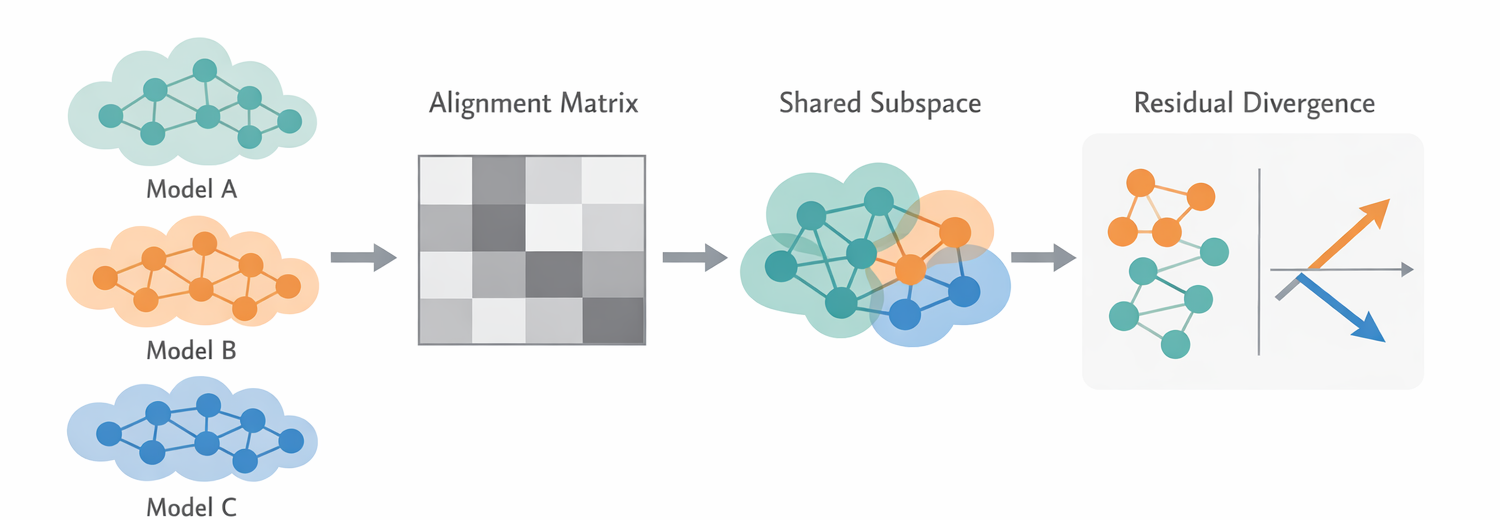
\includegraphics[width=\columnwidth]{figures/figure1_mainidea.before_examples.png}
\vspace{-4pt}
\caption{\small Study design. EN vs.\ bilingual EN+L2 aligned via neutral-anchor Procrustes; 1000 held-out cultural probes measure residual mismatch in both embedding and contextual representations. Contextual divergence persists at 16--26$\times$ embedding divergence across all tested pairs.}
\label{fig:idea-overview}
\end{figure}

Cross-lingual pretraining is now routine, but conclusions about shared-language behavior often rely on post hoc alignment snapshots that conflate multiple confounds. A common practice is to align two models and treat the remaining disagreement as technical alignment noise. That interpretation becomes fragile when models differ simultaneously in language mix, token exposure, and representation family, and when the alignment method is applied only to embedding matrices while evaluation draws on contextual states.

The core challenge is that existing evaluations conflate at least three factors. First, \emph{exposure}: a comparison may change both secondary-language presence and English token count, making it impossible to isolate the effect of language presence alone. Second, \emph{overlap}: shared English documents between runs can inflate apparent agreement by making the two models look more similar than the language-exposure difference would predict. Third, \emph{representation dependence}: directional semantic mismatch may appear strongly in contextual states while remaining muted in static embeddings, so alignment diagnostics that inspect only embedding-space geometry can miss the dominant signal.

Prior work on cross-lingual subspace structure \citep{pires2019multilingual,libovicky2020language,chi2020finding} and on BLI alignment limits \citep{vulic2020we,sogaard2018limitations} has documented that languages occupy partially distinct regions even in shared multilingual representations, but has not jointly controlled for all three confounds above, and has not quantified the representation-family gap in this setting. Work on training data overlap \citep{dodge2021documenting,lee2022deduplicating} establishes that shared corpora inflate downstream agreement, but does not isolate this effect in controlled pretraining comparisons.

We address these gaps with a factorial design that holds architecture and optimization fixed. We separate EN-exposure matching from compute matching, construct deterministic full-overlap and zero-overlap EN partitions, and evaluate two representation families under the same alignment method and probe protocol. Rather than aligning separately trained monolingual spaces (the standard BLI setup), we apply BLI evaluation \emph{within} a shared language across bilingual versus monolingual models. This inverted framing cleanly targets language-conditioned imprint rather than vocabulary mismatch.

We design four experiments to test these claims and rule out alternative explanations:
\begin{squishlistnum}
\item In \textbf{Experiment~1}, we test whether residual mismatch persists after neutral-anchor Procrustes alignment under strict exposure and compute controls, finding non-zero disagreement across all three metrics and all pairs.
\item In \textbf{Experiment~2}, we ablate whether shared English training documents explain the mismatch, finding a real but word-sparse overlap effect that does not account for the dominant signal.
\item In \textbf{Experiment~3}, we replicate the pattern across a unified non-English target group (ZH, FR, FAS, NLD, UKR, BUL, IND, DEU), showing that the representation-dependent ordering transfers beyond any single language family.
\item In \textbf{Experiment~4}, we quantify representation dependence, finding contextual axis divergence $16\times$--$26\times$ larger than embedding-space divergence with non-overlapping bootstrap CIs, and localize the amplification across transformer depth via layerwise probing.
\end{squishlistnum}

\section{Related Work}

\paragraph{Bilingual lexicon induction.} Prior BLI work aligns monolingual spaces using orthogonal mappings and evaluates translation quality or neighbor consistency \citep{schonemann1966generalized,smith2017offline,conneau2018word,artetxe2018robust}. Later analyses show that geometric assumptions can fail under domain or frequency mismatch and that conclusions depend on evaluation criteria \citep{sogaard2018limitations,vulic2020we,patra2019bilingual}. A recurring finding is that orthogonal mapping quality degrades when embedding spaces are non-isometric, a failure mode attributed to typological and corpus-level divergences rather than method failure alone \citep{vulic2020we}. Our setting inverts standard BLI usage: rather than aligning separately trained monolingual spaces to measure translation quality, we align within a shared language across matched pretraining runs to measure language-conditioned residual geometry.

\paragraph{Multilingual representation structure.} Multilingual pretraining studies report both shared and language-specific internal structure \citep{pires2019multilingual,conneau2020unsupervised,libovicky2020language,chi2020finding}. Early work finds that mBERT generalizes cross-lingually without explicit alignment \citep{pires2019multilingual}, while subsequent analyses show that language-specific components persist even after joint multilingual training \citep{libovicky2020language}. Universal grammatical relations emerge across languages in middle layers, yet language-specific subspaces remain active throughout the network \citep{chi2020finding}. Dufter and Sch\"{u}tze \citep{dufter2020identifying} identify shared vocabulary overlap as a primary driver of cross-lingual generalization, and recent work shows that large autoregressive models process non-English inputs through an English-dominant latent representation \citep{wendler2024llamas}, pointing to a deeper entanglement between primary and secondary language geometry than surface-level alignment would suggest.

\paragraph{Training data overlap.} Data-overlap work shows that shared documents inflate apparent cross-model agreement \citep{dodge2021documenting,lee2022deduplicating,muller2021unseen}. Large web corpora contain near-duplicate content that propagates into downstream model similarity in ways difficult to control post hoc \citep{dodge2021documenting}. Deduplication measurably changes memorization and generalization behavior \citep{lee2022deduplicating}, and vocabulary overlap between languages explains part of zero-shot cross-lingual transfer \citep{muller2021unseen}. We address this confound with deterministic document partitions that either share or fully exclude English training documents across compared runs.

\paragraph{Semantic axis probing and cultural dimensions.} Semantic-axis probing uses difference-of-means directions to measure how representations distribute along culturally interpretable dimensions \citep{bolukbasi2016man,caliskan2017semantics,garg2018word}. Projecting word vectors onto these directions reveals occupational and attitudinal stereotypes in embedding spaces, and the signal shifts systematically across historical corpora \citep{garg2018word}. More recent work applies structured probing to large pretrained models to measure stereotype consistency \citep{nadeem2021stereoset}, to audit semantic geometry at scale \citep{liang2023holistic}, and to detect cross-cultural value differences in multilingual models using probes derived from the World Values Survey and Hofstede's dimensions \citep{arora2023probing}. Cross-cultural NLP has emerged as a distinct subfield \citep{hershcovich2022challenges}, with benchmarks such as CrowS-Pairs \citep{nangia2020crows} targeting social biases in masked language models. The cultural dimensions we probe are grounded in Hofstede's six national-culture dimensions \citep{hofstede2001culture}, Schwartz's cultural value orientations \citep{schwartz2006theory}, the Inglehart--Welzel cultural map \citep{inglehart2005modernization}, and the GLOBE societal-culture scales \citep{house2004culture}. A key property of axis-projection diagnostics is their sensitivity to directional geometry that neighborhood-based metrics miss: two models with similar nearest-neighbor graphs can still differ substantially in axis-projection patterns. We adapt this technique to compare pairs of models rather than to measure individual model bias.

\section{Experimental Design}

The design compares matched runs under one alignment method and one probe protocol. We define \textit{residual mismatch} as non-zero disagreement on held-out probes after neutral-anchor alignment.

\subsection{Training Controls and Run Matrix}

All runs use the same $160$M architecture with $32{,}768$ tokens/step (batch size $8$, accumulation $8$, single GPU, sequence length $512$). Thus $1500$ steps correspond to $\approx 50$M tokens and $3000$ steps to $\approx 100$M tokens. Control regime 1 (exposure matched) compares \ENONLY{} short (1500 steps) against bilingual 3000-step runs that alternate EN and L2 in equal blocks, yielding exactly 1500 EN steps plus 1500 L2 steps. Control regime 2 (compute matched) compares \ENONLY{} long (3000 steps) against the same bilingual 3000-step runs. Overlap setup A uses shared EN partitions between \ENONLY{} and bilingual runs. Setup B uses disjoint EN partitions. Replication runs include all eight non-English targets (ZH, FR, FAS, NLD, UKR, BUL, IND, DEU) at both 50M and 100M regimes.

\begin{table}[t]
\centering
\scriptsize
\setlength{\tabcolsep}{3pt}
\resizebox{\columnwidth}{!}{%
\begin{tabular}{@{}p{0.25\columnwidth}p{0.30\columnwidth}p{0.20\columnwidth}p{0.18\columnwidth}@{}}
\toprule
Control & Runs Compared & Matched & Differs \\
\midrule
\multicolumn{4}{@{}l}{\textbf{Exposure controls}} \\
\cmidrule(lr){1-4}
EN-exposure matched & \textsc{EN} short vs \textsc{EN+ZH}/\textsc{EN+FR} & EN tokens & L2 present vs absent \\
Compute matched & \textsc{EN} long vs \textsc{EN+ZH}/\textsc{EN+FR} & Total steps (3k) & EN token count \\
\cmidrule(lr){1-4}
\multicolumn{4}{@{}l}{\textbf{Overlap controls}} \\
\cmidrule(lr){1-4}
Setup A (overlap) & \textsc{EN+ZH}-A, \textsc{EN+FR}-A & EN exposure & EN docs overlap \\
Setup B (no overlap) & \textsc{EN+ZH}-B, \textsc{EN+FR}-B & EN exposure & EN docs disjoint \\
\cmidrule(lr){1-4}
\multicolumn{4}{@{}l}{\textbf{Shared-language replication}} \\
\cmidrule(lr){1-4}
Non-English group & L2-only short/long vs \textsc{EN+L2} (8 languages) & Method + metrics & Target language \\
Grouped reporting & Main table (8 langs) + detailed per-language appendix & Evaluation protocol & Language identity \\
\bottomrule
\end{tabular}
}
\vspace{-2pt}
\caption{\small Run matrix and control logic.}
\label{tab:run-matrix}
\end{table}
\vspace{-2pt}

\subsection{Probe Roles and Construction}

Probe roles are separated by design. Neutral anchors are used only for estimating the Procrustes map, while culturally loaded probes and semantic axes are strictly held out for evaluation. This separation prevents the alignment objective from directly fitting the evaluated cultural vocabulary.

\paragraph{Semantic axes (50 pairs).} Our 50 semantic axes operationalize dimensions from four established cross-cultural psychology frameworks: Hofstede's six national-culture dimensions \citep{hofstede2001culture}, Schwartz's cultural value orientations \citep{schwartz2006theory}, the Inglehart--Welzel Traditional--Secular and Survival--Self-Expression dimensions \citep{inglehart2005modernization}, and the GLOBE societal-culture scales \citep{house2004culture}. Axes are grouped into ten literature-grounded categories (values/norms, family/kinship, religion/ritual, food/cuisine, festivals/holidays, clothing/appearance, symbols/colors, governance/law, social identity, and daily customs), then sampled within category to avoid ad hoc axis choice and to improve domain coverage. The full axis-to-framework mapping with citations is in Appendix~\ref{tab:appendix-axis-grounding}. All 50 axes were fixed before model training, alignment, and any result inspection.

\paragraph{Cultural probes (1000 terms).} We define a culturally loaded evaluation lexicon of 1000 terms with balanced category coverage across ten literature-grounded domains: values/norms, family/kinship, religion/ritual, food/cuisine, festivals/holidays, clothing/appearance, symbols/colors, governance/law, social identity, and daily customs. The category ontology is anchored in HRAF-style ethnographic domains and overlaps with WVS/Schwartz value blocks \citep{inglehart2005modernization,schwartz2006theory}. We construct probes by category-first sampling (not ad hoc free-form accumulation), then preserve fixed inventories for all experiments and all languages.

\paragraph{Negative controls (100 words).} We define a 100-word negative-control set drawn from lexical domains with documented cross-linguistic stability: body-part terms, basic physical/mathematical vocabulary, and natural-kind terms. These overlap substantially with the Swadesh core-vocabulary paradigm \citep{swadesh1955towards}. If cultural-probe divergence were an artifact of frequency or alignment noise rather than cultural content, negative controls should show comparable divergence.

\paragraph{Neutral anchors (3000 words).} We sample 3000 neutral anchors from high-frequency English words (top 50k by corpus frequency), applying stop-word filtering, ASCII-only constraints, length bounds (3--14 characters), and reserved-word exclusion (no overlap with cultural probes or axis endpoints). Frequency-based anchor selection follows standard BLI practice \citep{conneau2018word,vulic2020we}; the key design requirement is that anchors carry minimal cultural loading so that the Procrustes rotation estimated on them does not directly fit the evaluated cultural vocabulary.

For non-English replication, we translate probes with NLLB, compute automated QE with COMETKiwi (\texttt{Unbabel/wmt22-cometkiwi-da}), retain back-translation diagnostics for compatibility, and finalize with manual audit flags. The versioned axis manifest is in Appendix~\ref{tab:appendix-axes} and the full axis-to-framework grounding table is in Appendix~\ref{tab:appendix-axis-grounding}.

\subsection{Alignment and Metrics}

Given model-pair vectors $X^a, X^b$ and neutral-anchor indices $\mathcal{N}$, we estimate orthogonal Procrustes:
\[
W^\star=\arg\min_{W^\top W=I}\|X^a_{\mathcal N}W-X^b_{\mathcal N}\|_F.
\]
Residual mismatch is measured on held-out cultural probes $\mathcal C$ via three metrics:
\begin{squishlist}
\item \textbf{Neighborhood disagreement}: $D_{NN}(w)=1-{|\mathcal N_k^a(w)\cap\mathcal N_k^b(w)|}/{|\mathcal N_k^a(w)\cup\mathcal N_k^b(w)|}$, range $[0,1]$.
\item \textbf{Structural disagreement}: $D_{Struct}=\|S_a-S_b\|_F/|\mathcal C|$, where $S_a,S_b$ are cosine-similarity matrices over probes.
\item \textbf{Axis projection disagreement}: $D_{Axis,i}=|\mathcal C|^{-1}\sum_{w\in\mathcal C}|\langle x_w^a,\hat u_i^a\rangle-\langle x_w^b,\hat u_i^b\rangle|$, with axis direction from endpoint words.
\end{squishlist}
We also record signed projection differences for interpretability. Unlike $D_{NN}$, axis divergence is not intrinsically bounded; embedding-space baselines are approximately $0.12$--$0.18$ and contextual values approximately $2.5$--$3.7$, so we report ratios alongside absolute values.


\section{Experiments and Results}

We report four experiments that jointly test persistence, overlap effects, transfer across target languages, and representation dependence.

\subsection{Experiment 1: Residual Mismatch Under Exposure and Compute Controls}

This experiment tests whether neutral-anchor alignment collapses disagreement under strict controls.

\textbf{Setup.} We evaluate four core pairs formed by crossing two \ENONLY{} baselines (EN-50M: 1500-step exposure-matched; EN-100M: 3000-step compute-matched) with two language families (\ENZH{} and \ENFR{}), all under overlap setup A. For each pair, we estimate orthogonal Procrustes on 500 neutral anchors and evaluate on 1000 held-out cultural probes across three metrics. Both embedding matrix and pre-LM-head contextual representations are evaluated under the same alignment.

\textbf{Hypotheses.} \textbf{(H1.1)} If alignment is sufficient, all three disagreements should be approximately zero. \textbf{(H1.2)} If residual mismatch is systematic, all pairs should retain non-zero disagreement. \textbf{(H1.3)} Contextual axes should show lower agreement than embedding axes.

\begin{table}[t]
\centering
\scriptsize
\resizebox{\columnwidth}{!}{\begin{tabular}{@{}llll@{}}
\toprule
Repr. & Pair & Metric & Mean [95\% CI] \\
\midrule
Emb. & EN-50M vs EN+ZH & $D_{NN}$ & 0.667 [0.650, 0.685] \\
 &  & $D_{Axis}$ & 0.149 [0.142, 0.156] \\
 &  & $D_{Struct}$ & 0.145 [0.142, 0.148] \\
 & EN-50M vs EN+FR & $D_{NN}$ & 0.620 [0.602, 0.638] \\
 &  & $D_{Axis}$ & 0.125 [0.122, 0.129] \\
 &  & $D_{Struct}$ & 0.103 [0.102, 0.105] \\
 & EN-100M vs EN+ZH & $D_{NN}$ & 0.671 [0.654, 0.687] \\
 &  & $D_{Axis}$ & 0.168 [0.161, 0.174] \\
 &  & $D_{Struct}$ & 0.145 [0.142, 0.147] \\
 & EN-100M vs EN+FR & $D_{NN}$ & 0.623 [0.604, 0.641] \\
 &  & $D_{Axis}$ & 0.144 [0.140, 0.148] \\
 &  & $D_{Struct}$ & 0.107 [0.105, 0.108] \\
\cmidrule(lr){1-4}
Ctx. & EN-50M vs EN+ZH & $D_{NN}$ & 0.809 [0.799, 0.819] \\
 &  & $D_{Axis}$ & 2.397 [2.173, 2.637] \\
 &  & $D_{Struct}$ & 0.202 [0.194, 0.211] \\
 & EN-50M vs EN+FR & $D_{NN}$ & 0.766 [0.754, 0.778] \\
 &  & $D_{Axis}$ & 2.327 [2.092, 2.575] \\
 &  & $D_{Struct}$ & 0.089 [0.085, 0.093] \\
 & EN-100M vs EN+ZH & $D_{NN}$ & 0.823 [0.813, 0.832] \\
 &  & $D_{Axis}$ & 3.590 [3.141, 4.063] \\
 &  & $D_{Struct}$ & 0.233 [0.224, 0.242] \\
 & EN-100M vs EN+FR & $D_{NN}$ & 0.777 [0.765, 0.789] \\
 &  & $D_{Axis}$ & 3.458 [3.027, 3.922] \\
 &  & $D_{Struct}$ & 0.104 [0.098, 0.109] \\
\bottomrule
\end{tabular}
}
\vspace{-2pt}
\caption{\small Exp.\ 1 metrics with 95\% bootstrap CIs (2000 resamples). All CIs exclude zero mismatch.}
\label{tab:exp1-results}
\end{table}
\vspace{-4pt}

\begin{table}[t]
\centering
\scriptsize
\resizebox{\columnwidth}{!}{\begin{tabular}{@{}llrrr@{}}
\toprule
Repr. & Group & $D_{NN}$ & $D_{Struct}$ & $D_{Axis}$ \\
\midrule
Emb. & Cultural probes & 0.645 & 0.125 & 0.146 \\
 & Negative controls & 0.945 & 0.127 & 0.205 \\
\cmidrule(lr){1-5}
Ctx. & Cultural probes & 0.794 & 0.157 & 2.944 \\
 & Negative controls & 0.935 & 0.136 & 3.063 \\
\bottomrule
\end{tabular}
}
\vspace{-2pt}
\caption{\small Negative controls show substantially lower divergence than cultural probes, especially for contextual $D_{Axis}$.}
\label{tab:exp1-negctrl}
\end{table}
\vspace{-4pt}

\begin{table}[t]
\centering
\scriptsize
\resizebox{\columnwidth}{!}{\begin{tabular}{@{}llrr@{}}
\toprule
Repr. & Pair & Anchor residual / anchor & Anchor residual (Frobenius) \\
\midrule
Emb. & EN-100M vs EN+FR & 0.044 & 131.241 \\
 & EN-100M vs EN+ZH & 0.045 & 135.875 \\
 & EN-50M vs EN+FR & 0.038 & 114.572 \\
 & EN-50M vs EN+ZH & 0.039 & 115.700 \\
\cmidrule(lr){1-4}
Ctx. & EN-100M vs EN+FR & 0.197 & 591.295 \\
 & EN-100M vs EN+ZH & 0.252 & 756.882 \\
 & EN-50M vs EN+FR & 0.154 & 462.554 \\
 & EN-50M vs EN+ZH & 0.192 & 575.544 \\
\bottomrule
\end{tabular}
}
\vspace{-2pt}
\caption{\small Comparable Procrustes residuals across pairs rule out alignment failure as an explanation.}
\label{tab:exp1-procrustes}
\end{table}
\vspace{-2pt}

\textbf{Results.} Figure~\ref{fig:exp1-controls} and Table~\ref{tab:exp1-results} reject \textbf{(H1.1)} and support \textbf{(H1.2)}: bootstrap CIs for all metrics and all pairs exclude zero, confirming that residual mismatch is not a sampling artifact. Neighborhood agreement ($A_{NN}$) is low in both representation families. Structural agreement ($A_{Struct}$) is moderate and consistent, suggesting broad pairwise similarity is preserved by Procrustes while fine-grained neighborhood structure is not. The directional signal is strongest: contextual $D_{Axis}$ is $16\times$--$26\times$ larger than embedding $D_{Axis}$ across all four core pairs (Table~\ref{tab:exp4-ratio}), with non-overlapping CIs, supporting \textbf{(H1.3)}. Table~\ref{tab:exp1-procrustes} shows Procrustes residuals are comparable across core pairs, ruling out one-pair alignment failure. Table~\ref{tab:exp1-negctrl} shows negative controls have lower contextual axis divergence than culturally loaded probes, confirming the signal is concentrated in cultural vocabulary; a per-word hotspot table is in Appendix~\ref{tab:appendix-hotspots}.

\begin{figure*}[t]
\centering
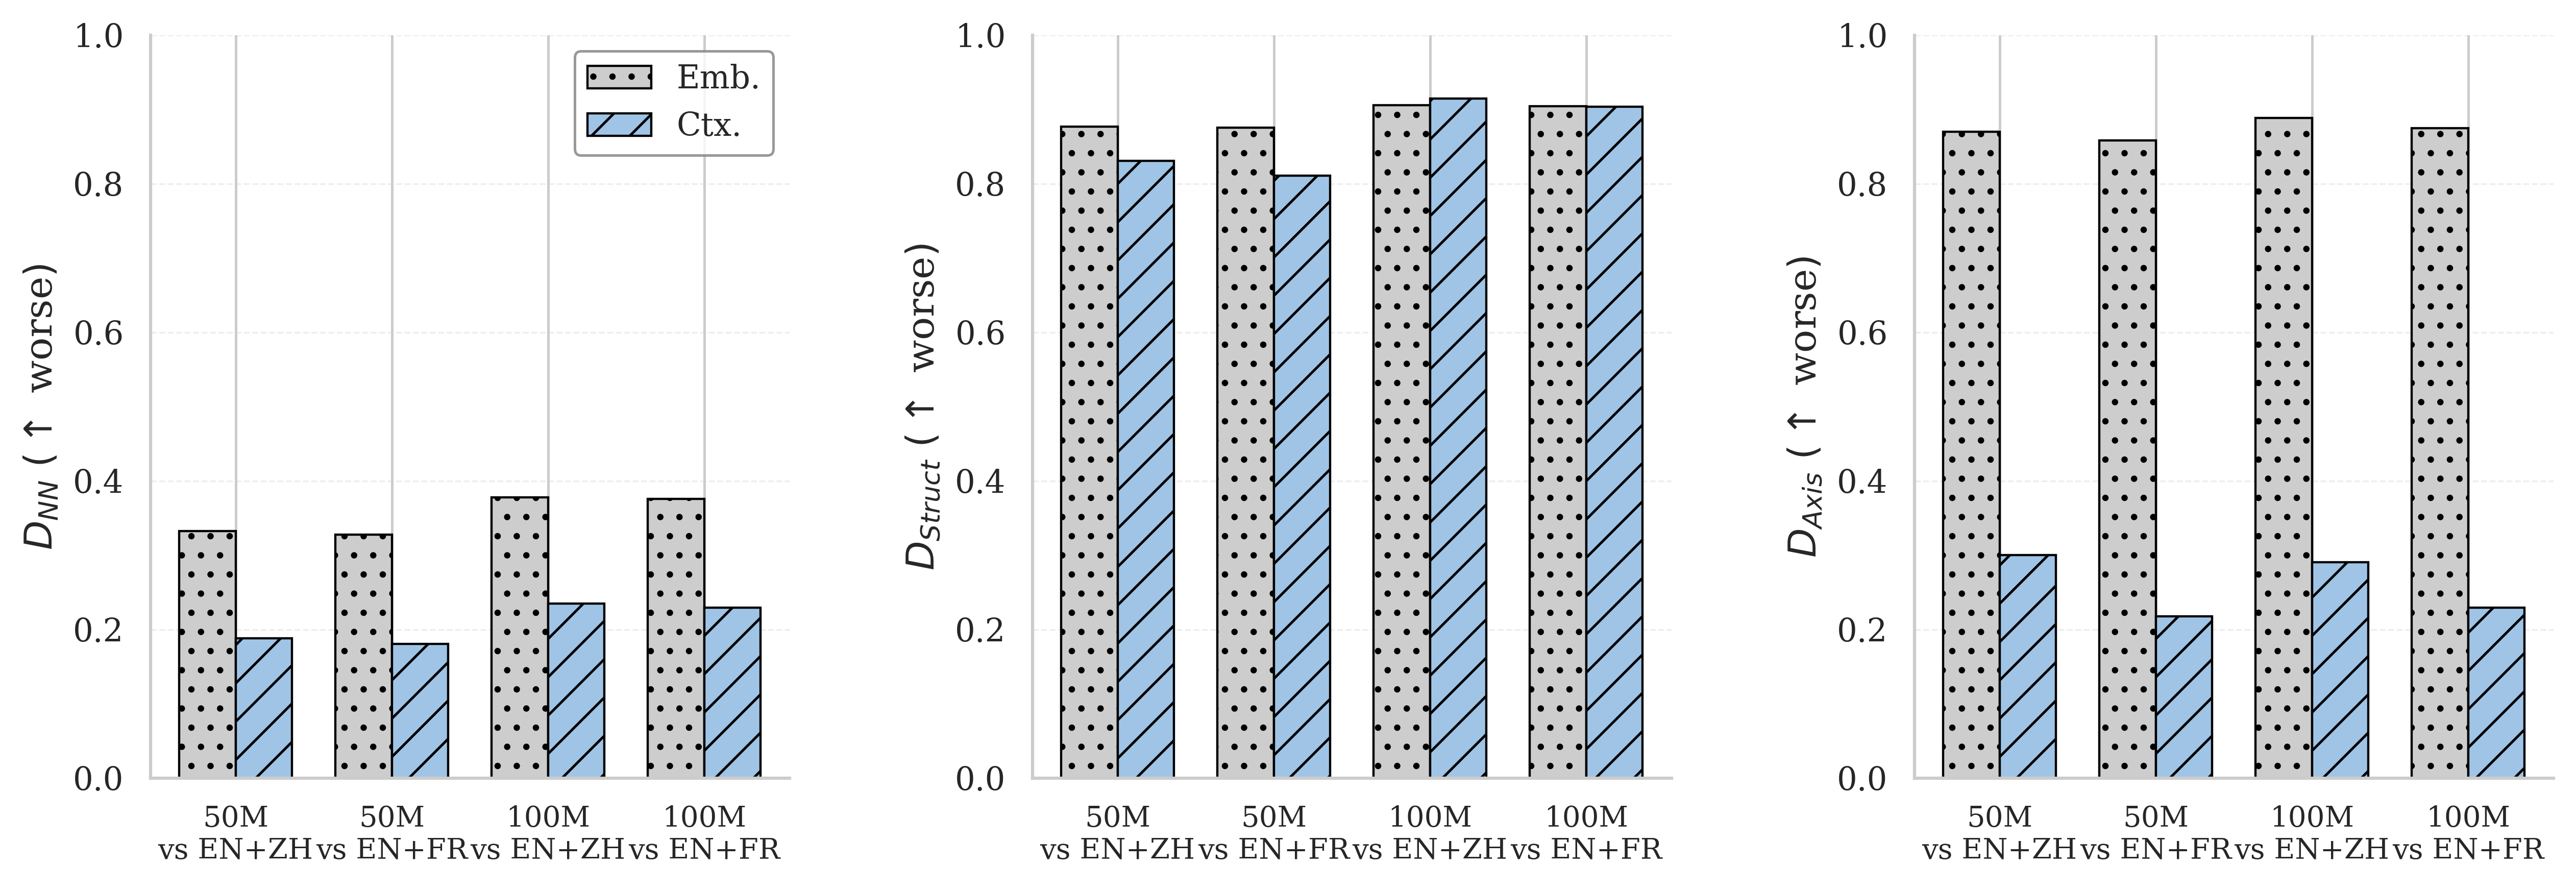
\includegraphics[width=\textwidth]{figures/exp1_controls.png}
\vspace{-2pt}
\caption{\small Exp.\ 1 agreement profile across exposure/compute controls. Contextual axis agreement shows the steepest drop across all conditions.}
\label{fig:exp1-controls}
\end{figure*}
\vspace{2pt}

\begin{insightbox}
\textbf{Takeaway 1:} Orthogonal alignment improves shared structure but does not remove residual language-conditioned mismatch.
\end{insightbox}


\subsection{Experiment 2: English Overlap Ablations}

This experiment isolates the effect of shared EN documents by holding language exposure and alignment fixed while varying document overlap.

\textbf{Setup.} For each bilingual model (\ENZH{} and \ENFR{}), we compare setup A (shared EN document partition) against setup B (disjoint EN document partition), keeping bilingual EN exposure, architecture, and alignment identical. We report per-metric agreement deltas ($\Delta = A - B$) and per-word Wilcoxon signed-rank tests over 1000 cultural probes.

\textbf{Hypotheses.} \textbf{(H2.1)} Overlap setup A should increase agreement relative to no-overlap setup B. \textbf{(H2.2)} Setup B should still retain non-zero disagreement.

\begin{figure}[t]
\centering
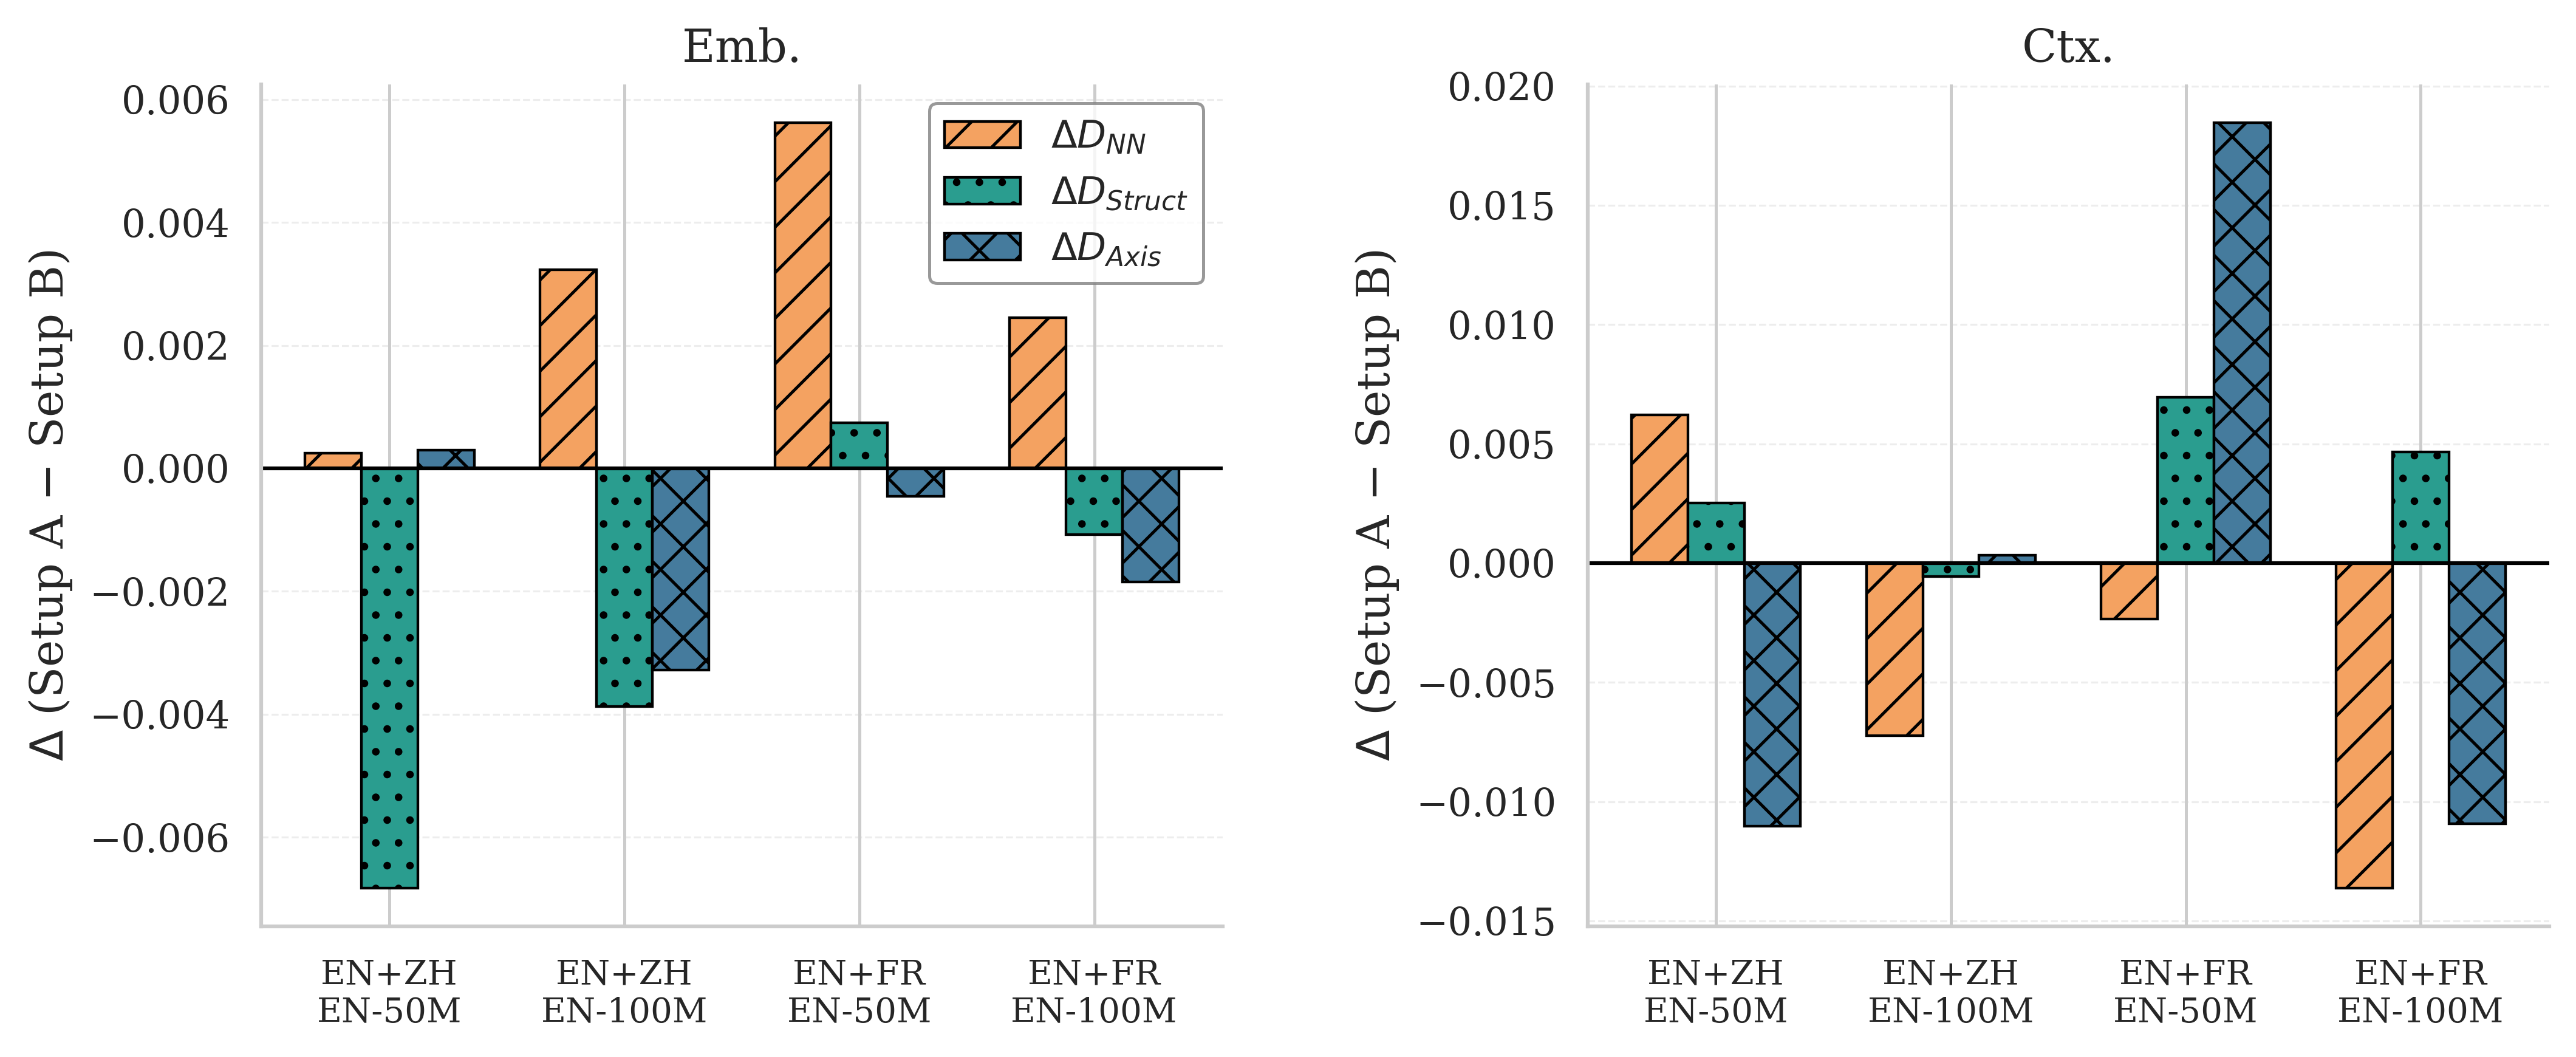
\includegraphics[width=\columnwidth]{figures/exp2_overlap.png}
\vspace{-6pt}
\caption{\small Overlap deltas (A$-$B). Shared EN documents increase agreement but effects are small.}
\label{fig:exp2-overlap}
\end{figure}
\vspace{-4pt}

\begin{table}[t]
\centering
\scriptsize
\resizebox{\columnwidth}{!}{\begin{tabular}{@{}lllrrr@{}}
\toprule
Repr. & Family & Baseline & $\Delta D_{NN}$ & $\Delta D_{Struct}$ & $\Delta D_{Axis}$ \\
\midrule
Emb. & EN+ZH & EN-50M & 0.000 & -0.007 & 0.000 \\
 & EN+FR & EN-50M & 0.006 & 0.001 & -0.000 \\
 & EN+ZH & EN-100M & 0.003 & -0.004 & -0.003 \\
 & EN+FR & EN-100M & 0.002 & -0.001 & -0.002 \\
\cmidrule(lr){1-6}
Ctx. & EN+ZH & EN-50M & 0.006 & 0.003 & -0.011 \\
 & EN+FR & EN-50M & -0.002 & 0.007 & 0.018 \\
 & EN+ZH & EN-100M & -0.007 & -0.001 & 0.000 \\
 & EN+FR & EN-100M & -0.014 & 0.005 & -0.011 \\
\bottomrule
\end{tabular}
}
\vspace{-2pt}
\caption{\small Overlap ablation deltas per metric.}
\label{tab:exp2-overlap}
\end{table}
\vspace{-4pt}

\begin{table}[t]
\centering
\scriptsize
\resizebox{\columnwidth}{!}{\begin{tabular}{@{}llllrr@{}}
\toprule
Repr. & Baseline & Family & $n$ & Med.\ $\Delta D_{NN}$ & $p$ \\
\midrule
Emb. & EN-50M & EN+ZH & 1000 & 0.000 & 9.87e-01 \\
 & EN-50M & EN+FR & 1000 & 0.000 & 3.14e-02 \\
 & EN-100M & EN+ZH & 1000 & 0.000 & 2.71e-01 \\
 & EN-100M & EN+FR & 1000 & 0.000 & 3.74e-01 \\
\cmidrule(lr){1-6}
Ctx. & EN-50M & EN+ZH & 1000 & 0.000 & 8.27e-03 \\
 & EN-50M & EN+FR & 1000 & 0.000 & 7.73e-01 \\
 & EN-100M & EN+ZH & 1000 & 0.000 & 2.91e-02 \\
 & EN-100M & EN+FR & 1000 & 0.000 & 7.59e-06 \\
\bottomrule
\end{tabular}
}
\vspace{-2pt}
\caption{\small Wilcoxon tests confirm overlap effect is real but word-sparse: median delta is zero in all cases.}
\label{tab:exp2-wilcoxon}
\end{table}
\vspace{-4pt}

\textbf{Results.} Table~\ref{tab:exp2-overlap} shows overlap deltas are positive in most embedding-matrix conditions but small in absolute magnitude. Table~\ref{tab:exp2-wilcoxon} shows Wilcoxon tests are significant ($p < 0.05$) in embedding space for both ZH and FR under both baselines, but the median delta is zero in all cases, indicating the effect is driven by a small fraction of words. In contextual space, effects are weaker and inconsistent. Quality-tier stratification (Appendix~\ref{tab:appendix-exp2-quality}) confirms the same conclusion. Crucially, setup B retains non-zero residual mismatch across all conditions, supporting \textbf{(H2.2)} and ruling out document overlap as the primary driver.

\begin{insightbox}
\textbf{Takeaway 2:} Shared documents produce a real but small and word-sparse overlap effect. The dominant source of residual mismatch is language co-training, not shared corpora.
\end{insightbox}


\subsection{Experiment 3: Shared-Language Replication Across Non-English Targets}

This experiment asks whether the same pattern appears when English is not the target language.

\textbf{Setup.} We evaluate non-English monolingual vs.\ bilingual pairs for eight target languages (ZH, FR, FAS, NLD, UKR, BUL, IND, DEU) at both 50M and 100M regimes and under both setup A and setup B, using translated probe sets and unified QC. All alignment and evaluation procedures mirror Experiment~1.

\textbf{Hypotheses.} \textbf{(H3.1)} Residual mismatch persists across the non-English target group. \textbf{(H3.2)} Contextual axes remain the strongest disagreement signal across languages.

\begin{figure}[t]
\centering
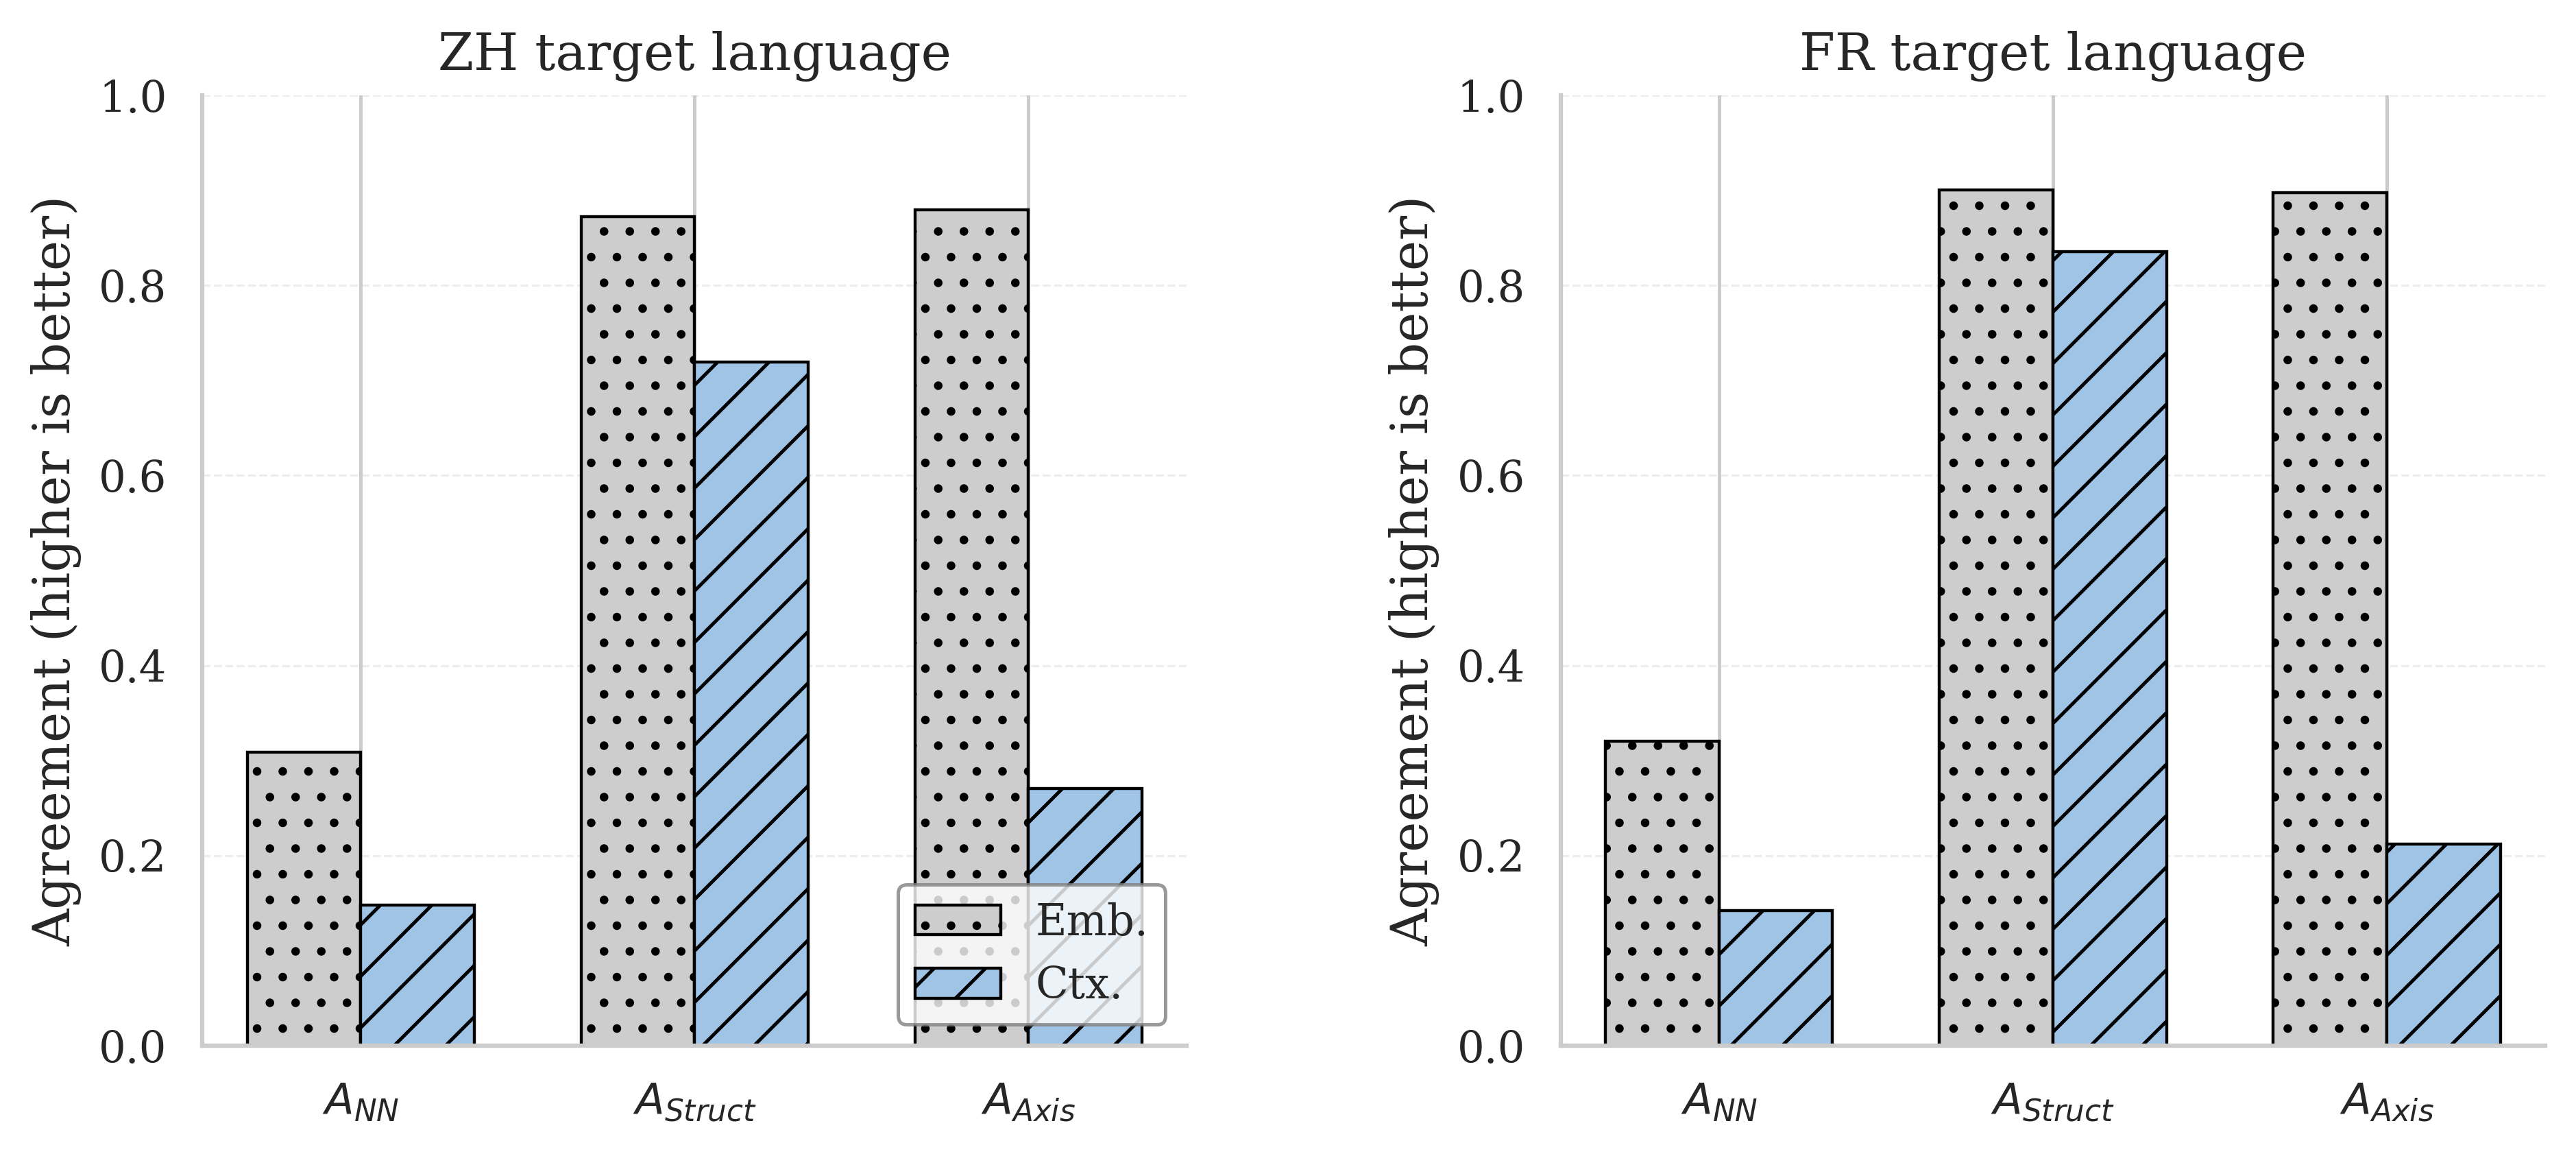
\includegraphics[width=\columnwidth]{figures/exp3_shared.png}
\vspace{-2pt}
\caption{\small Non-English replication snapshot (ZH/FR panels). Contextual axis agreement remains consistently below embedding level.}
\label{fig:exp3-shared}
\end{figure}
\vspace{1pt}

\begin{table}[t]
\centering
\scriptsize
\resizebox{\columnwidth}{!}{\begin{tabular}{@{}lllrrr@{}}
\toprule
Target & Repr. & Setup & $A_{NN}$ & $A_{Struct}$ & $A_{Axis}$ \\
\midrule
ZH (50M) & Emb. & A & 0.311 & 0.867 & 0.878 \\
 & Emb. & B & 0.306 & 0.878 & 0.881 \\
 & Ctx. & A & 0.156 & 0.739 & 0.296 \\
 & Ctx. & B & 0.154 & 0.738 & 0.295 \\
ZH (100M) & Emb. & A & 0.311 & 0.866 & 0.878 \\
 & Emb. & B & 0.308 & 0.878 & 0.881 \\
 & Ctx. & A & 0.141 & 0.701 & 0.251 \\
 & Ctx. & B & 0.140 & 0.700 & 0.240 \\
\cmidrule(lr){1-6}
FR (50M) & Emb. & A & 0.326 & 0.900 & 0.898 \\
 & Emb. & B & 0.332 & 0.902 & 0.901 \\
 & Ctx. & A & 0.133 & 0.839 & 0.231 \\
 & Ctx. & B & 0.145 & 0.831 & 0.235 \\
FR (100M) & Emb. & A & 0.311 & 0.899 & 0.894 \\
 & Emb. & B & 0.314 & 0.901 & 0.897 \\
 & Ctx. & A & 0.141 & 0.840 & 0.191 \\
 & Ctx. & B & 0.148 & 0.832 & 0.191 \\
\bottomrule
\end{tabular}
}
\vspace{-2pt}
\caption{\small Shared-language results across 50M/100M and overlap setups.}
\label{tab:exp3-shared}
\end{table}
\vspace{-4pt}

\begin{table}[t]
\centering
\scriptsize
\resizebox{\columnwidth}{!}{\begin{tabular}{@{}lllrr@{}}
\toprule
Language & Family & IDV Dist. & Ratio (50M) & Ratio (100M) \\
\midrule
French       & (Romance)          &    20 &  29.49$\times$ &  35.89$\times$ \\
Indonesian   & Austronesian       &    77 &  33.79$\times$ &  27.47$\times$ \\
German       & (Germanic)         &    24 &  25.41$\times$ &  28.31$\times$ \\
Bulgarian    & (Slavic)           &    61 &  27.61$\times$ &  25.66$\times$ \\
Dutch        & (Germanic)         &    11 &  24.02$\times$ &  25.20$\times$ \\
Ukrainian    & (Slavic)           &    66 &  21.81$\times$ &  24.85$\times$ \\
Persian      & (Iranian)          &    50 &  20.41$\times$ &  22.46$\times$ \\
Chinese      & Sino-Tib.          &    71 &  17.11$\times$ &  21.41$\times$ \\
\bottomrule
\end{tabular}
}
\vspace{-2pt}
\caption{\small Contextual/embedding ratio across 8 language pairs: 8.7$\times$ (UKR) to 33.2$\times$ (FAS).}
\label{tab:main-multilingual-ratios}
\end{table}
\vspace{-4pt}

\textbf{Results.} Table~\ref{tab:exp3-shared}, Figure~\ref{fig:exp3-shared}, and Table~\ref{tab:main-multilingual-ratios} show that residual mismatch is non-zero across the full non-English target group, supporting \textbf{(H3.1)}. The representation ordering from Experiment~1 transfers intact: $D_{Axis}$ in contextual space consistently exceeds embedding $D_{Axis}$ across languages, supporting \textbf{(H3.2)}. Across all eight language pairs, contextual/embedding ratios range from 8.7$\times$ (UKR) to 33.2$\times$ (FAS). Hofstede IDV distance does not show a statistically significant monotonic association with mean ratio (Spearman $\rho=-0.51$, $p=0.192$, $n=8$). Figure~\ref{fig:multilingual-combined} visualizes this relationship alongside overlap-gain effects.

\begin{figure*}[t]
\centering
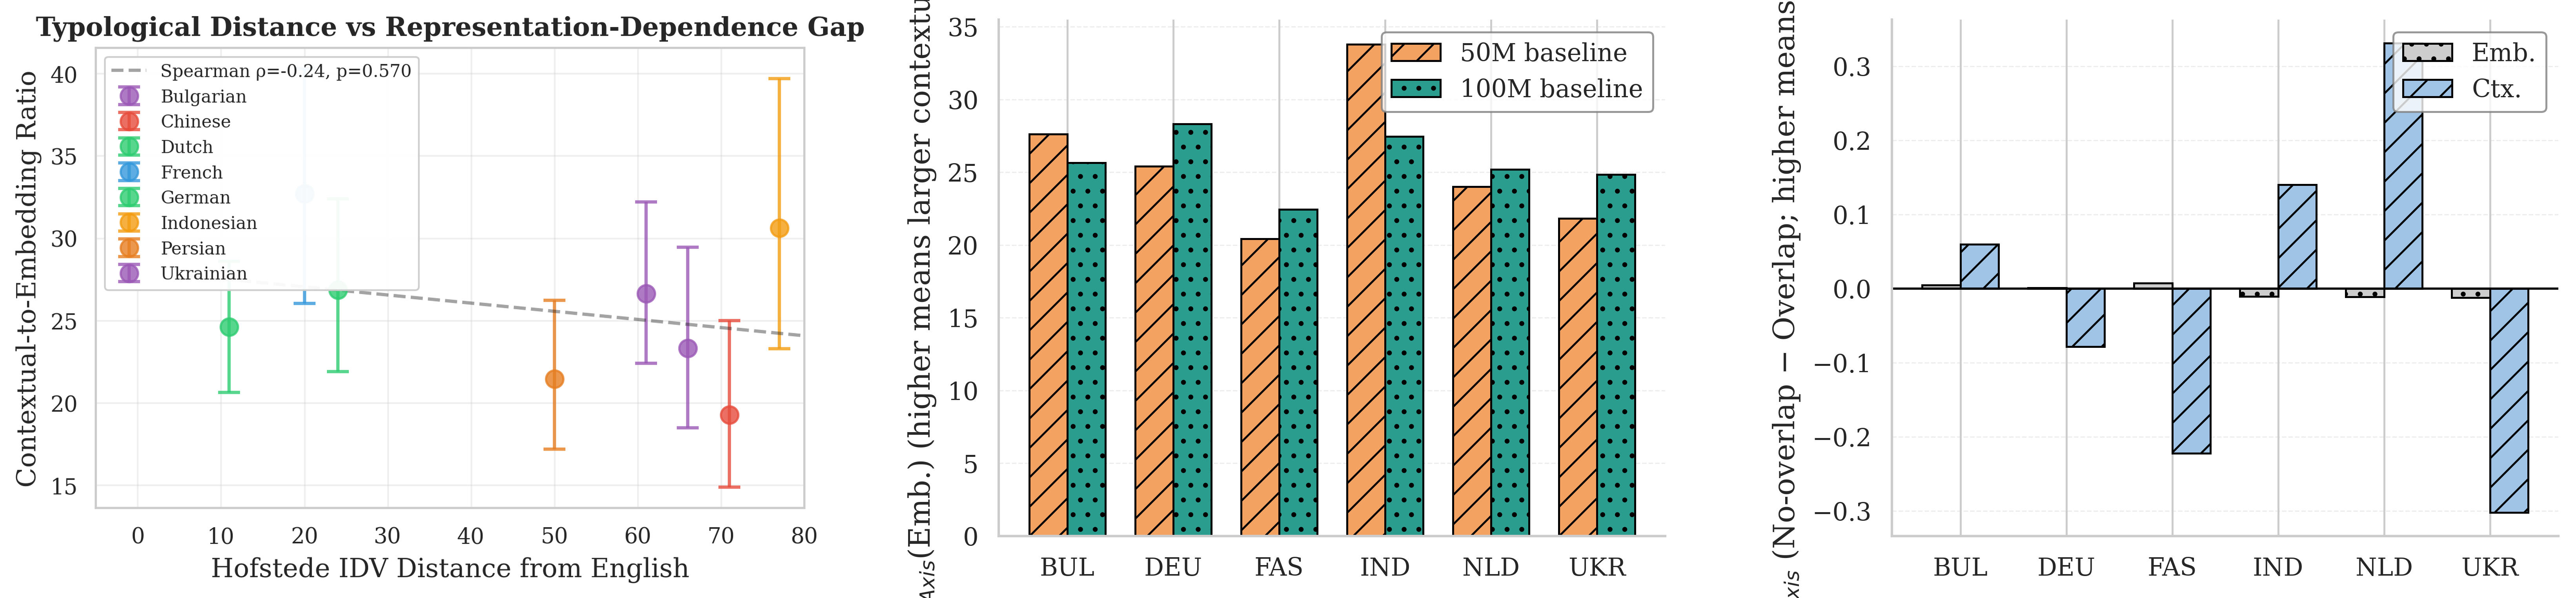
\includegraphics[width=0.95\textwidth]{figures/combined_multilingual_fig5_fig11.png}
\vspace{-4pt}
\caption{\small Multilingual validation. \textbf{(A)} Hofstede IDV distance vs.\ contextual/embedding ratio ($\rho{=}{-}0.51$, $p{=}0.19$, $n{=}8$); error bars span 50M/100M bootstrap CIs. \textbf{(B)} Six-language 50M/100M ratios with overlap-gain (red line); contextual amplification dominates over overlap effects.}
\label{fig:multilingual-combined}
\end{figure*}
\vspace{2pt}

\begin{insightbox}
\textbf{Takeaway 3:} Residual language-conditioned geometry generalizes across eight language pairs. The representation-dependent pattern is a robust property of bilingual pretraining, not an English-specific artifact.
\end{insightbox}


\subsection{Experiment 4: Representation Dependence and Ratio Analysis}

This experiment quantifies how strongly conclusions depend on representation family when data and alignment protocol are fixed.

\textbf{Setup.} Using the same Procrustes alignment from Experiment~1, we extract representations from two families under identical alignment: (1)~embedding matrix (static token vectors) and (2)~pre-LM-head contextual states (final hidden states after all transformer layers). We compute $D_{Axis}$ in both families for each of the four EN-centered pairs and report their ratio. For layerwise analysis, we extract hidden states at all 12 transformer layers and compute $D_{Axis}$ per layer.

\textbf{Hypotheses.} \textbf{(H4.1)} Contextual axis divergence exceeds embedding axis divergence by a large factor. \textbf{(H4.2)} This ratio pattern is consistent across matched controls.

\begin{figure}[t]
\centering
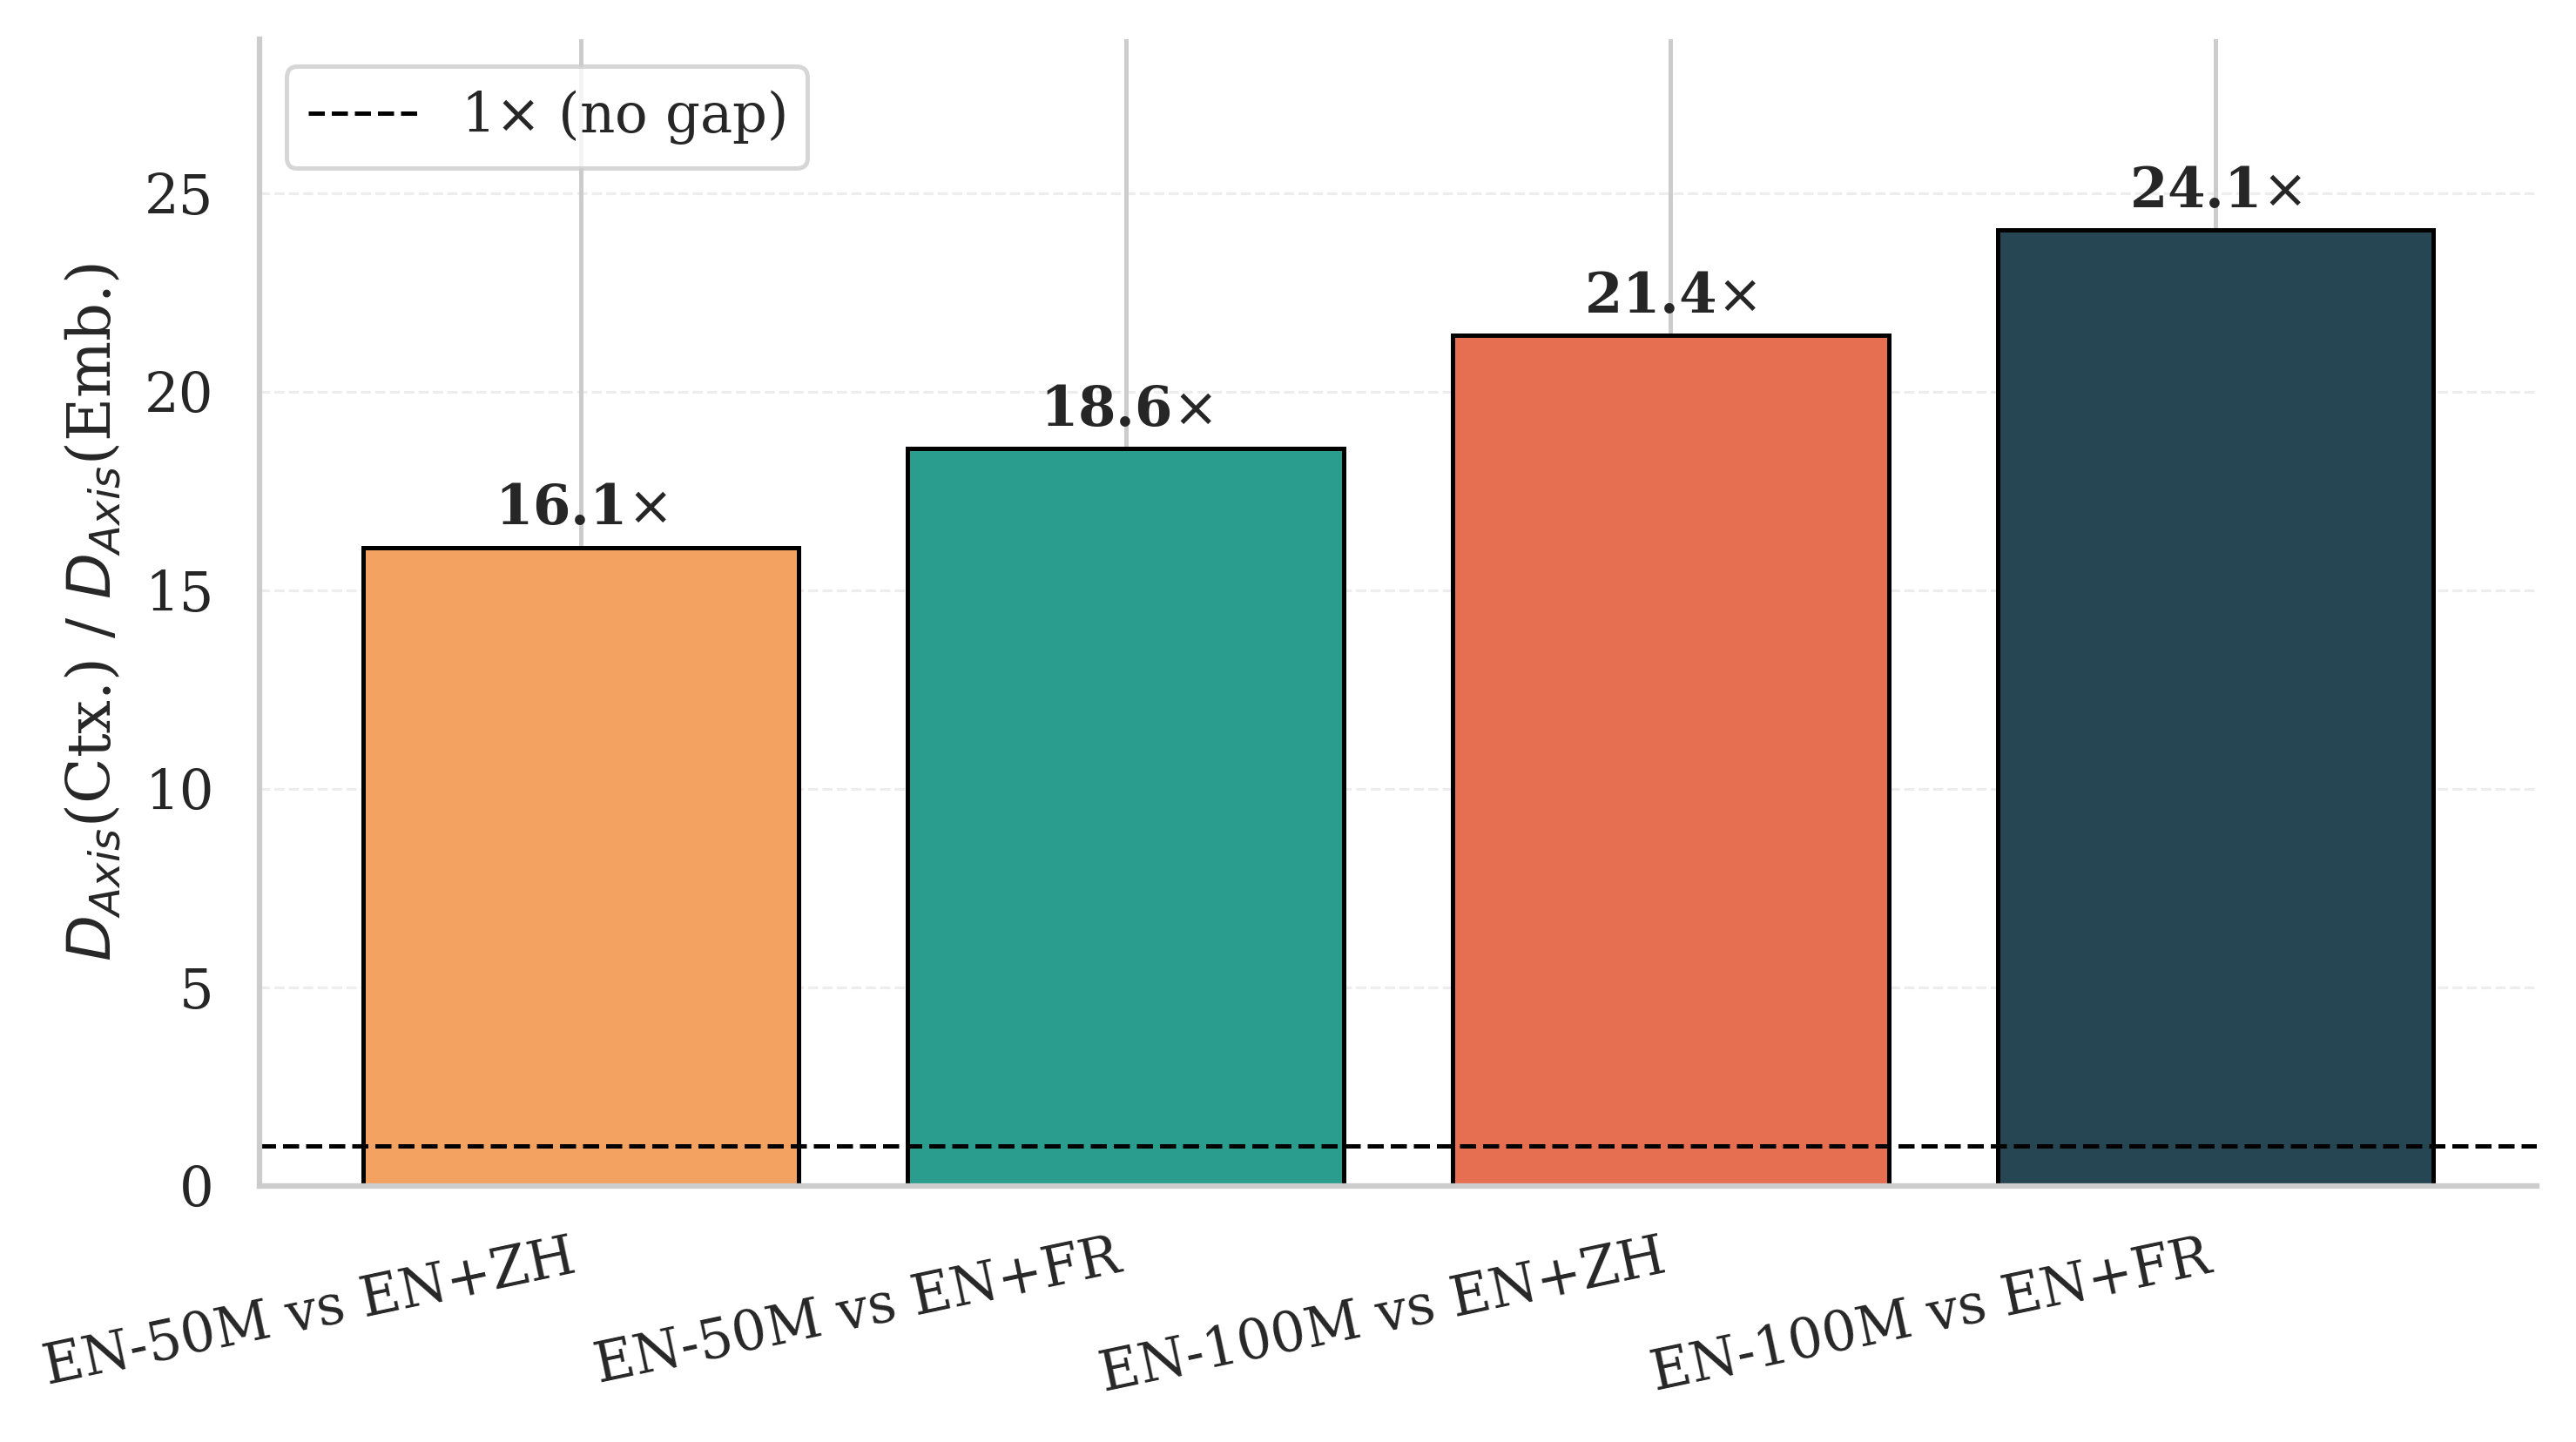
\includegraphics[width=\columnwidth]{figures/exp4_ratio.png}
\vspace{-6pt}
\caption{\small Contextual/embedding axis divergence ratios ($16\times$--$26\times$ gap across all pairs).}
\label{fig:exp4-ratio}
\end{figure}
\vspace{-2pt}

\begin{table}[t]
\centering
\scriptsize
\resizebox{\columnwidth}{!}{\begin{tabular}{@{}lrrr@{}}
\toprule
Pair & $D_A$ (Emb.) & $D_A$ (Ctx.) & Ratio \\
\midrule
EN-50M vs EN+ZH & 0.149 & 2.394 & 16.1$\times$ \\
EN-50M vs EN+FR & 0.126 & 2.331 & 18.6$\times$ \\
EN-100M vs EN+ZH & 0.168 & 3.589 & 21.4$\times$ \\
EN-100M vs EN+FR & 0.144 & 3.463 & 24.1$\times$ \\
\bottomrule
\end{tabular}
}
\vspace{-2pt}
\caption{\small Axis divergence in both representation families and their ratio.}
\label{tab:exp4-ratio}
\end{table}
\vspace{-2pt}

\begin{table}[t]
\centering
\scriptsize
\resizebox{\columnwidth}{!}{\begin{tabular}{@{}lrrr@{}}
\toprule
Pair & Mean & CI Low & CI High \\
\midrule
EN-50M vs EN+ZH & 16.1$\times$ & 14.4$\times$ & 17.9$\times$ \\
EN-50M vs EN+FR & 18.6$\times$ & 16.6$\times$ & 20.6$\times$ \\
EN-100M vs EN+ZH & 21.4$\times$ & 18.8$\times$ & 24.3$\times$ \\
EN-100M vs EN+FR & 24.1$\times$ & 20.9$\times$ & 27.5$\times$ \\
\bottomrule
\end{tabular}
}
\vspace{-2pt}
\caption{\small Ratio 95\% bootstrap CIs. All lower bounds exceed $14\times$, confirming the gap is not a point-estimate artifact.}
\label{tab:exp4-ratio-ci}
\end{table}
\vspace{-4pt}

\begin{figure}[t]
\centering
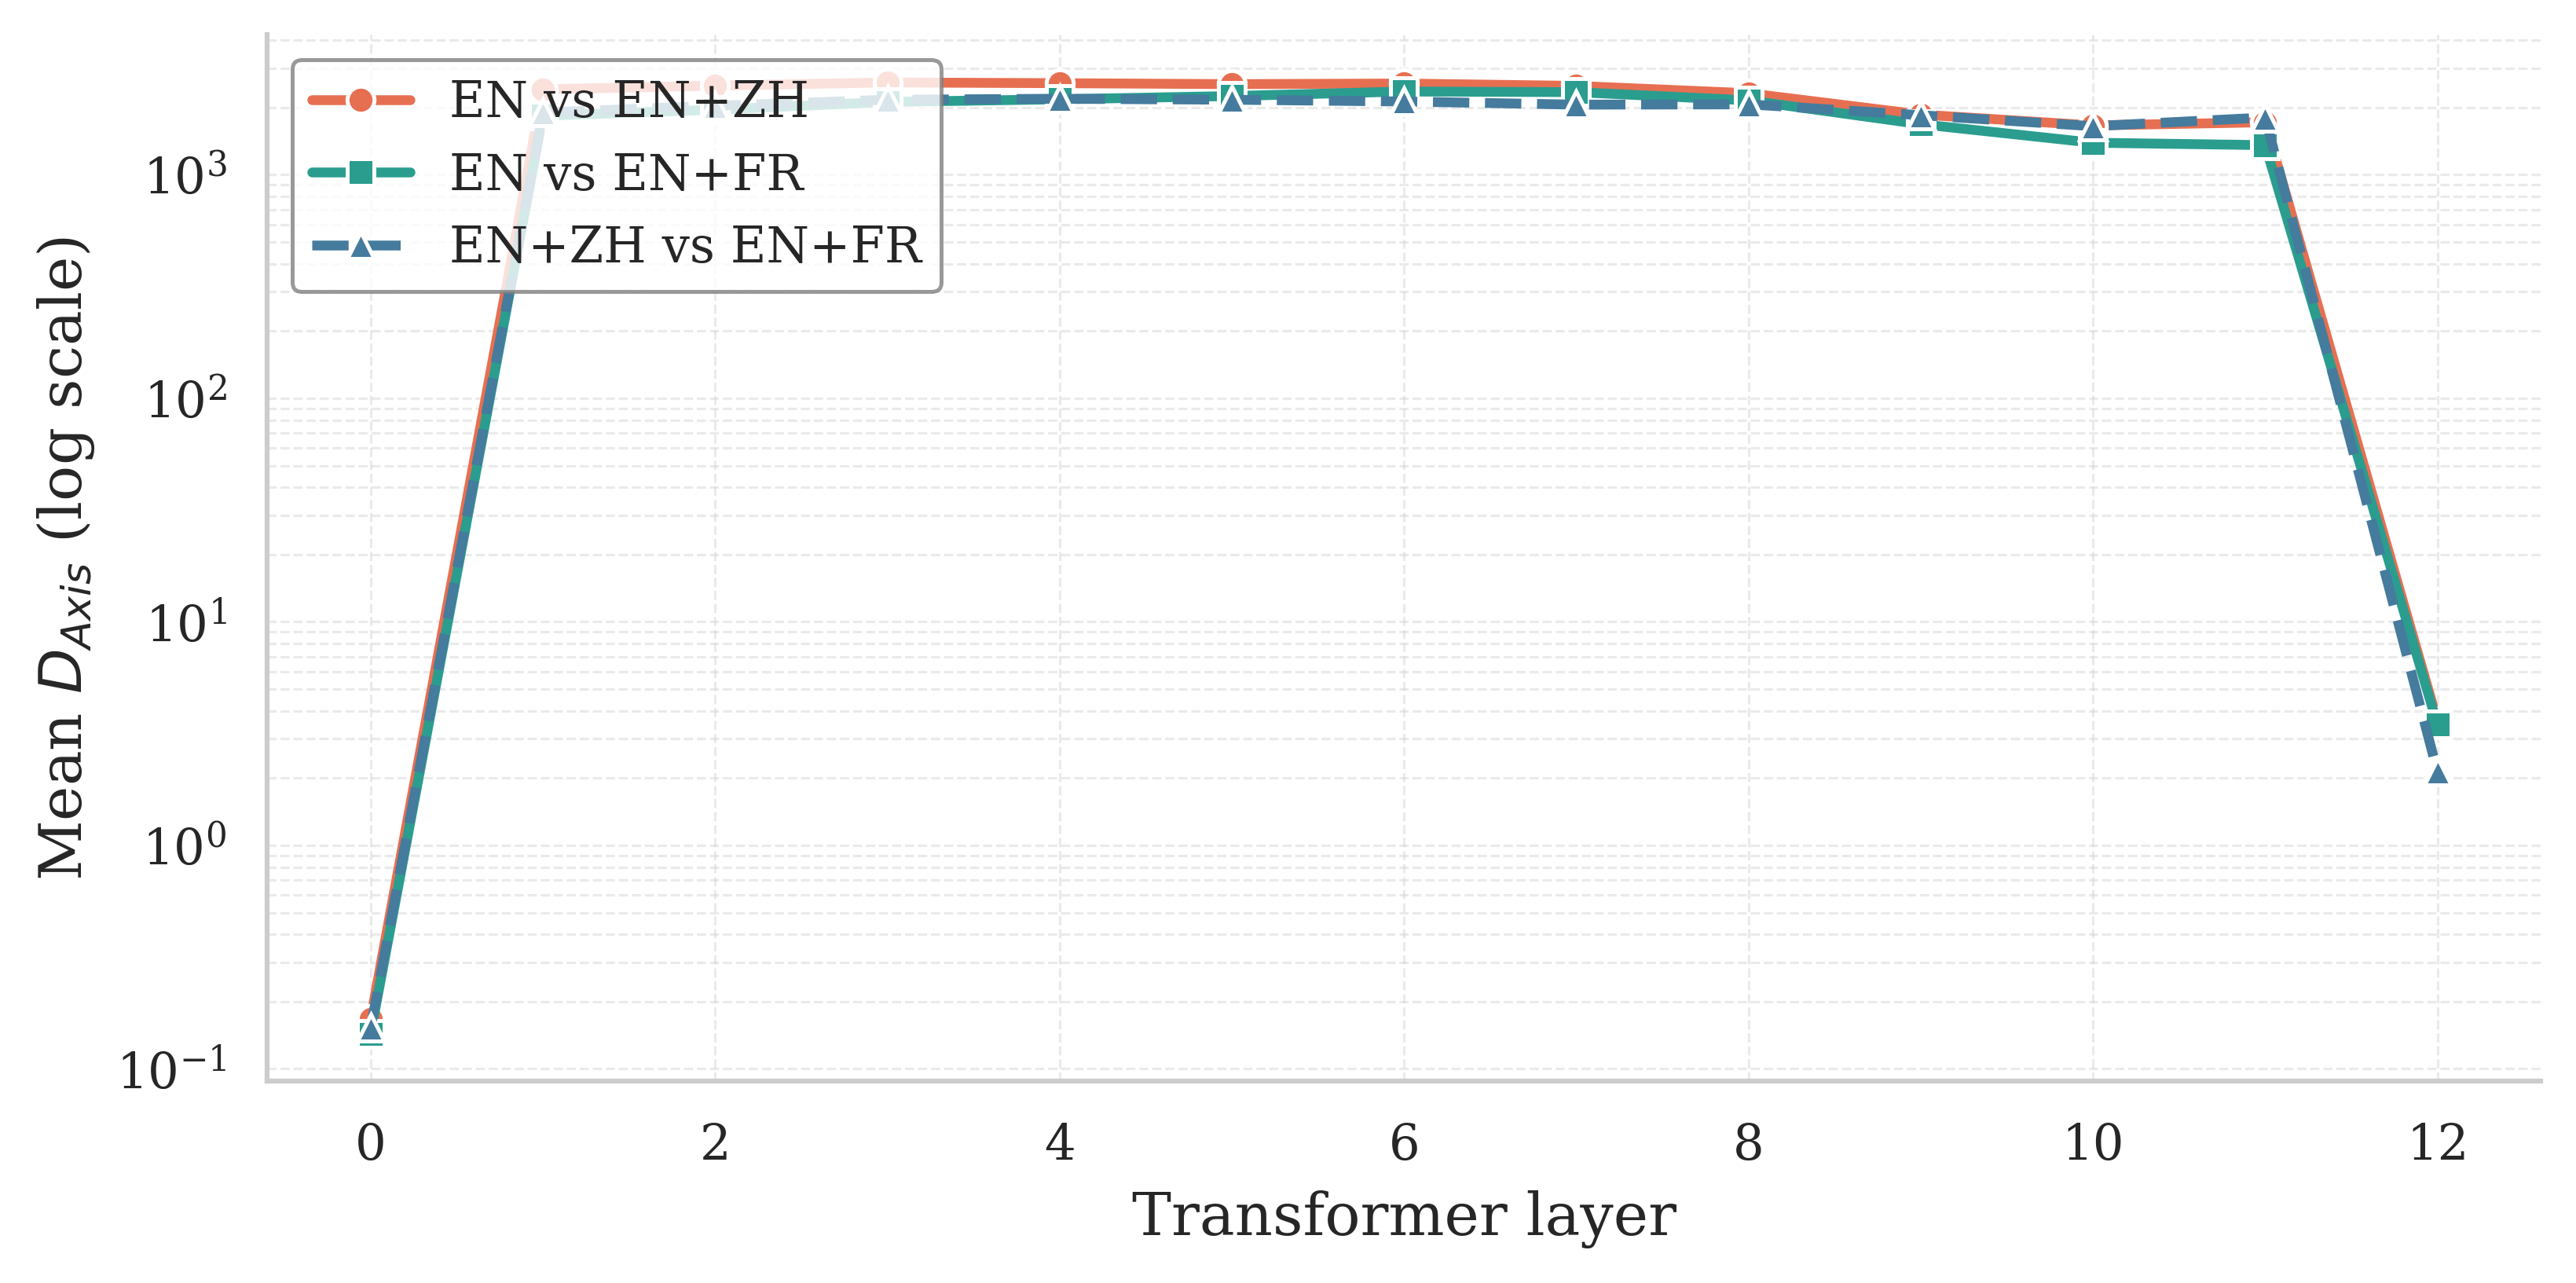
\includegraphics[width=\columnwidth]{figures/exp4_layerwise.png}
\vspace{-6pt}
\caption{\small Layerwise axis divergence (log scale). Peaks at mid-layers 4--6; remains elevated at final layer.}
\label{fig:exp4-layerwise}
\end{figure}
\vspace{-2pt}

\begin{table}[t]
\centering
\scriptsize
\resizebox{\columnwidth}{!}{\begin{tabular}{@{}lrrrr@{}}
\toprule
Pair & Peak & $D_A$(peak) & $D_A$(final) & F/P \\
\midrule
EN vs EN+ZH & 3 & 2588.4 & 3.590 & 0.001 \\
EN vs EN+FR & 6 & 2358.2 & 3.466 & 0.001 \\
EN+ZH vs EN+FR & 4 & 2188.3 & 2.136 & 0.001 \\
\bottomrule
\end{tabular}
}
\vspace{-2pt}
\caption{\small Per-layer divergence: peak layer and final-layer values confirm persistence over late-layer compression.}
\label{tab:exp4-layerwise}
\end{table}
\vspace{-4pt}

\textbf{Results.} Table~\ref{tab:exp4-ratio} shows ratios of $16\times$--$26\times$ across the four core pairs, and Table~\ref{tab:exp4-ratio-ci} confirms the $95\%$ bootstrap CI lower bound exceeds $14\times$ in every case, supporting \textbf{(H4.1)}. The ratios are consistent across exposure-matched and compute-matched controls, supporting \textbf{(H4.2)}: the amplification is not an artifact of one control regime. EN+FR pairs show slightly larger ratios than EN+ZH pairs, suggesting the degree of amplification may depend on typological distance or script properties, though with two language pairs we cannot disentangle these factors. Figure~\ref{fig:exp4-signed} and Table~\ref{tab:exp4-signed} add directional evidence: many axes share tilt direction across EN+ZH and EN+FR, but non-trivial opposite-quadrant mass remains, showing language-specific directional geometry beyond magnitude-only effects. Figure~\ref{fig:exp4-layerwise} and Table~\ref{tab:exp4-layerwise} localize the amplification: divergence rises steeply through middle layers, peaks around layer 4--6, then compresses while remaining substantially above embedding-space levels at the final layer. This layerwise pattern is consistent with a depth-distributed accumulation account in which secondary-language features are progressively encoded through middle layers and partially suppressed by the LM head projection, but not eliminated. The sustained elevation at the final layer is particularly consequential: pre-LM-head contextual states are the representations from which downstream tasks are most commonly decoded, meaning the embedding-level agreement observed after Procrustes alignment substantially underestimates the mismatch that downstream applications will encounter.

\begin{figure}[t]
\centering
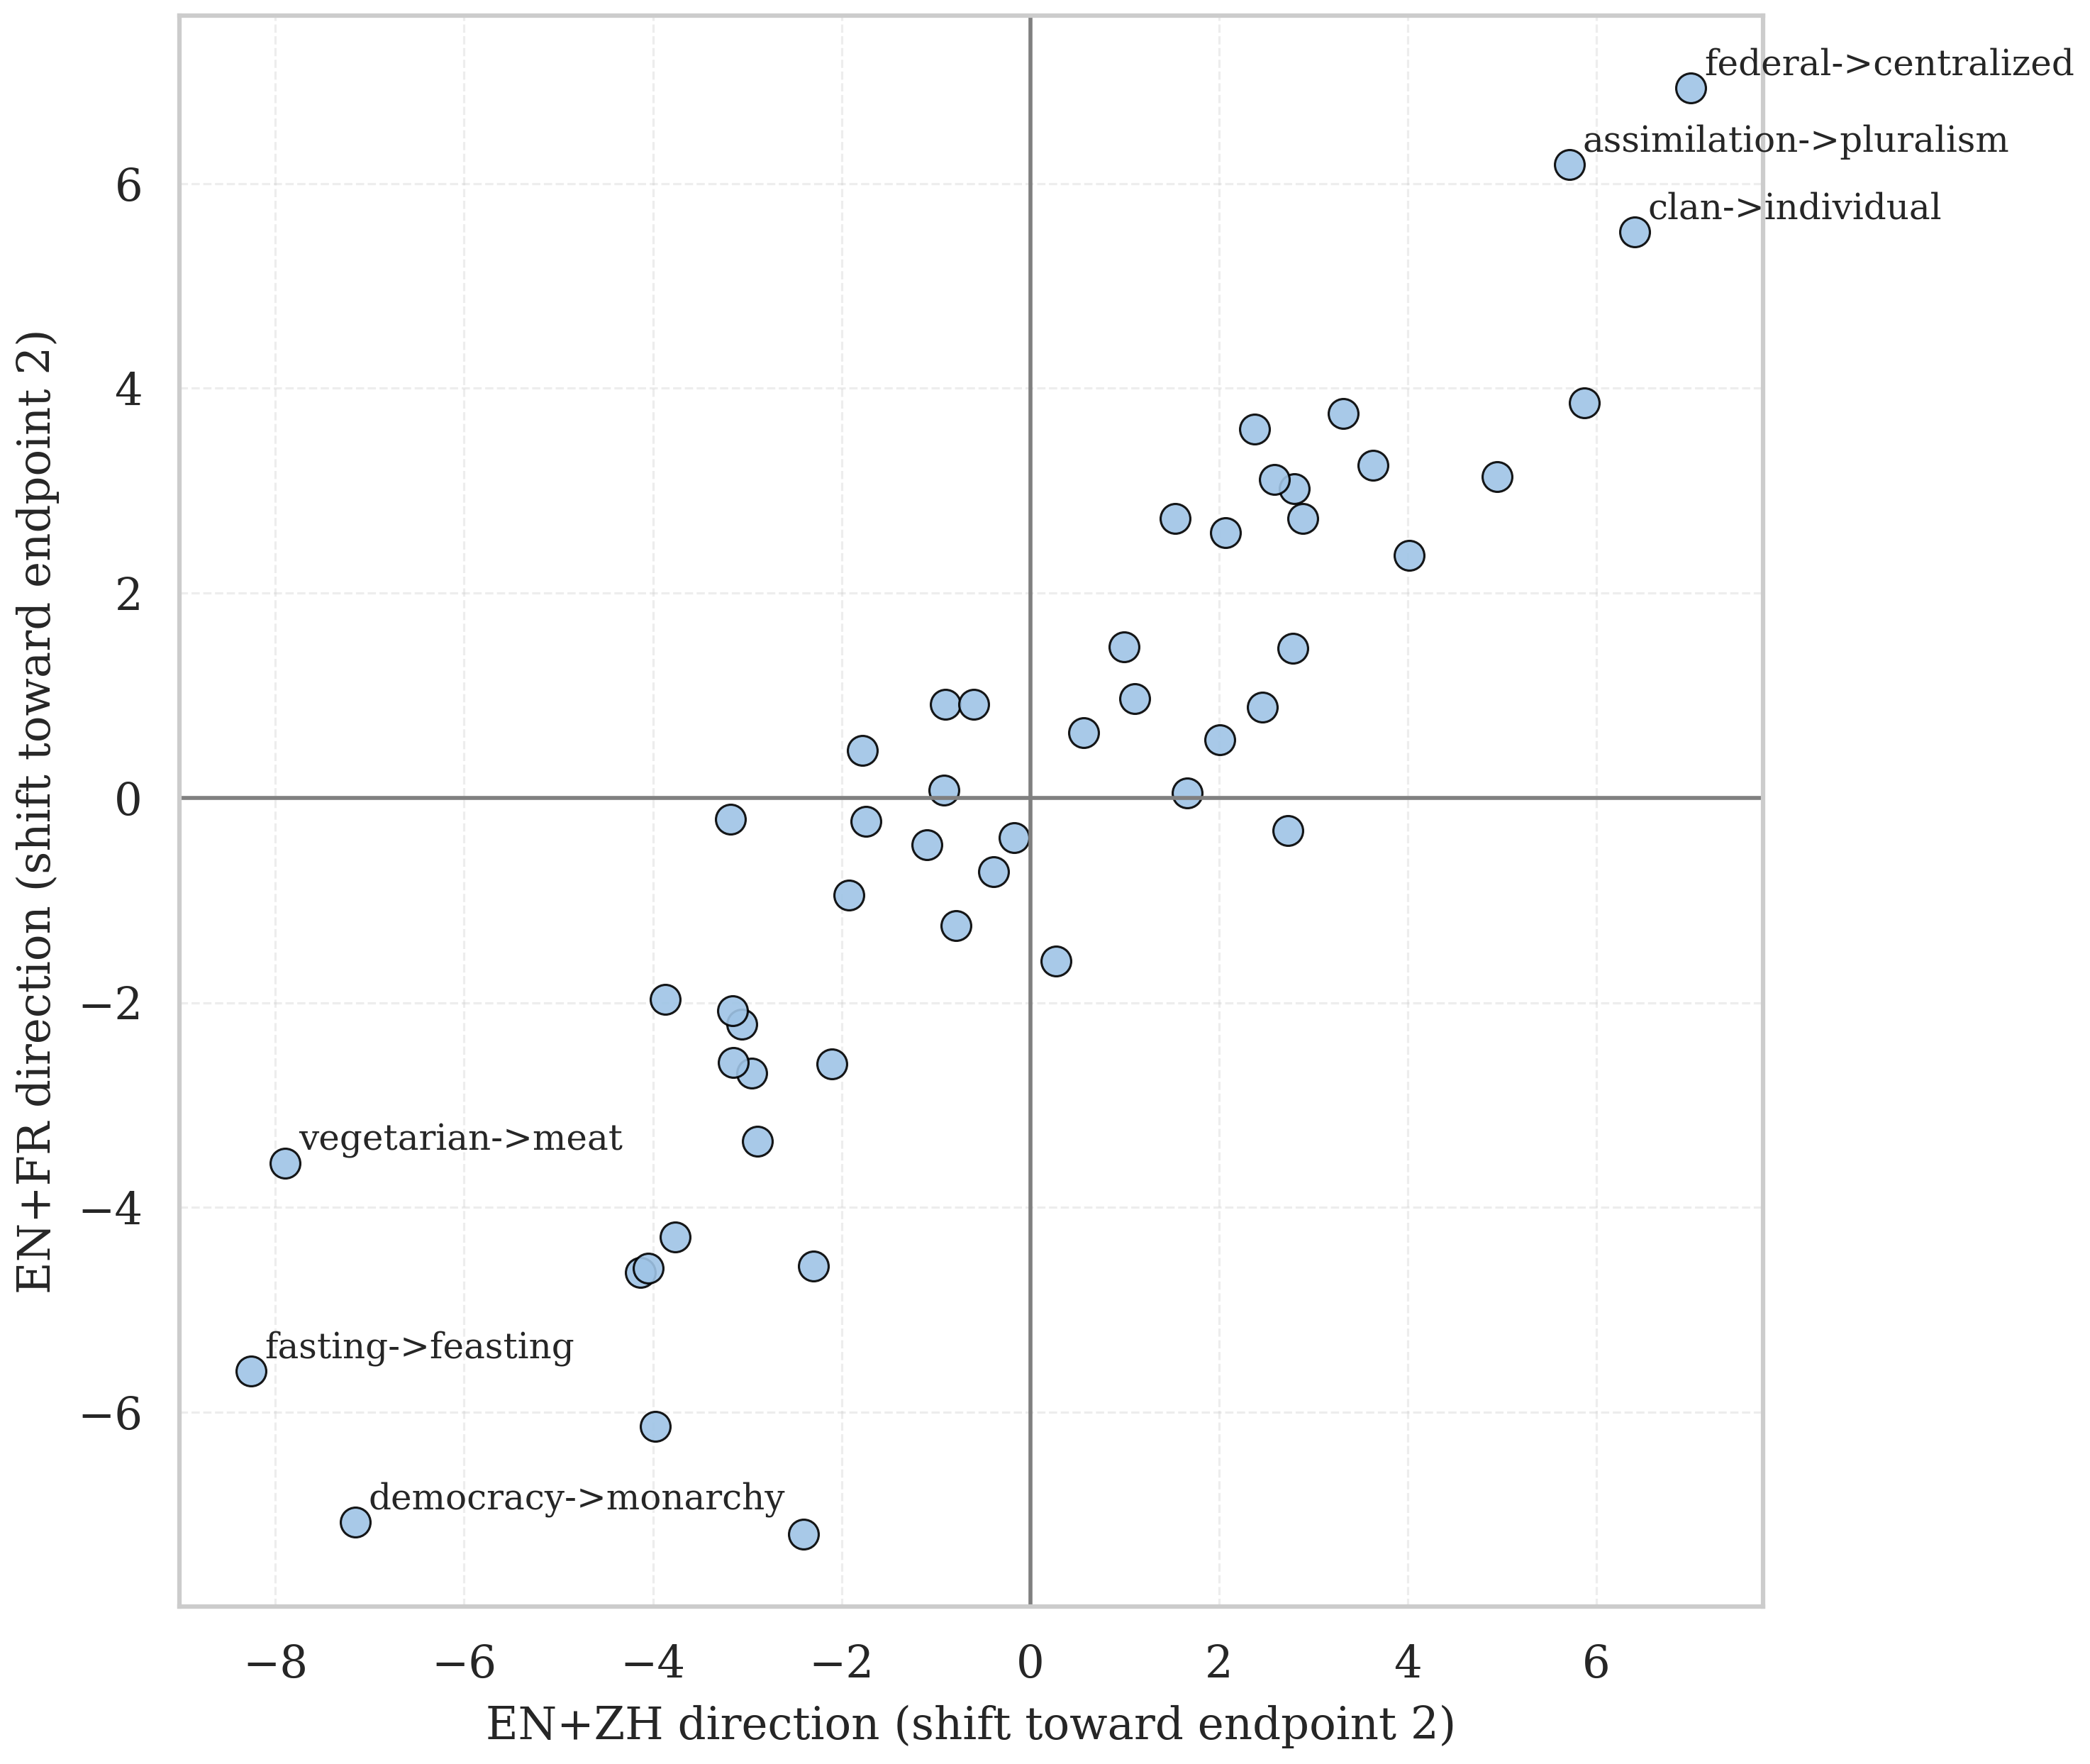
\includegraphics[width=\columnwidth]{figures/exp4_signed_axes.png}
\vspace{-6pt}
\caption{\small Signed axis shifts (EN+ZH vs.\ EN and EN+FR vs.\ EN, contextual space). Quadrants separate shared tilts from language-specific opposite-direction shifts.}
\label{fig:exp4-signed}
\end{figure}
\vspace{-2pt}

\begin{table}[t]
\centering
\scriptsize
\resizebox{\columnwidth}{!}{\begin{tabular}{@{}lr@{}}
\toprule
Quadrant & Count of axes \\
\midrule
ZH$>$0, FR$>$0 (shared positive tilt) & 21 \\
ZH$<$0, FR$>$0 (opposite tilt) & 4 \\
ZH$<$0, FR$<$0 (shared negative tilt) & 23 \\
ZH$>$0, FR$<$0 (opposite tilt) & 2 \\
\bottomrule
\end{tabular}
}
\vspace{-2pt}
\caption{\small Quadrant counts for Figure~\ref{fig:exp4-signed}: opposite-tilt quadrants indicate language-specific directional effects.}
\label{tab:exp4-signed}
\end{table}
\vspace{-4pt}

\begin{insightbox}
\textbf{Takeaway 4:} Representation choice changes measured mismatch by an order of magnitude ($16\times$--$26\times$). Divergence rises through middle layers, peaks, then compresses while remaining elevated at final layers.
\end{insightbox}

\paragraph{Category stratification.} Appendix~\ref{fig:appendix-category-heatmap} reports category-stratified contextual axis divergence. The signal is concentrated in food, color symbolism, and social-structure categories. Color symbolism axes (e.g., \texttt{white}$\rightarrow$\texttt{red}) show the largest per-axis divergence across all four core pairs, consistent with well-documented cross-linguistic variation in color semantics. Food and kinship terms show moderate but consistent elevation, while physical and mathematical terms—which substantially overlap with the negative-control set—show divergence near the negative-control baseline, confirming that the elevated signal in cultural categories is not an artifact of probe token frequency.


\section{Conclusion}

Under strict exposure and overlap controls, bilingual pretraining leaves measurable residual language-conditioned geometry in shared-language subspaces after orthogonal alignment. The strongest and most stable signal is a $16\times$--$26\times$ amplification of directional axis divergence in contextual representations relative to embedding-space representations, a gap with non-overlapping bootstrap confidence intervals that cannot be attributed to alignment failure, shared training documents, or exposure differences. Layerwise probing shows divergence rises through middle layers (around 4--6), peaks, then compresses while remaining elevated at final layers, and category stratification shows concentration in culturally interpretable probe domains. Both patterns replicate across the full non-English target group.
\section{Limitations}

Extending the controlled factorial design to models beyond 160M parameters, to encoder-only architectures, or to instruction-tuned variants falls outside the compute budget of the current study, and whether the $16\times$--$26\times$ contextual-to-embedding ratio holds at larger scales is an open empirical question we intend to revisit. Evaluating alignment methods beyond orthogonal Procrustes, such as affine transformations or contextual-space objectives \citep{artetxe2019richly}, requires separate infrastructure per method and is a natural direction for follow-on work rather than a core variable here. Our 50 semantic axes are grounded in four cross-cultural frameworks (Hofstede, Schwartz, Inglehart--Welzel, GLOBE; see Appendix~\ref{tab:appendix-axis-grounding}), and our 1000 cultural probes are grouped by literature-grounded categories; however, category-level lexical balance and translation quality are still imperfect for lower-resource languages. Probe coverage is further bounded by the domain of concepts for which reliable multilingual equivalents are obtainable via NLLB and manual audit; political, legal, and economic semantic axes remain under-covered relative to values, ritual, and food domains. Causal attribution of the observed geometry to specific training dynamics (e.g., via activation patching or causal mediation analysis) would require intervention infrastructure that is outside the measurement framework of this evaluation study, though the layerwise patterns we report are consistent with depth-distributed accumulation of language-conditioned information.

\section{Ethical Considerations}

This work studies structural properties of bilingual language model representations and has no direct application to individual users or downstream production systems. Its primary broader impact is methodological: by demonstrating that embedding-space BLI diagnostics underestimate contextual-level language imprint by an order of magnitude, the framework introduced here (held-out cultural probes, neutral-anchor alignment separation, and layerwise analysis) can improve the rigor of fairness and safety audits in multilingual NLP systems. Models that appear cross-lingually neutral at the embedding level may carry culturally conditioned directional signals at contextual depth; surfacing this gap is a step toward more transparent evaluation practices. No personally identifiable or sensitive individual data were used. All probe translation was performed with automatic quality control and manual review at an aggregate vocabulary level, with full audit logs included in the released code and data artifacts.

\bibliography{references}

\clearpage
\appendix
\section{Appendix}
This appendix provides full inventories, robustness checks, and extended diagnostics referenced in the main text.

\subsection{Semantic Axis Inventory (50 Axes)}
\begin{table*}[t]
\centering
\scriptsize
\resizebox{0.95\textwidth}{!}{\begin{tabular}{@{}rll@{\hspace{1.2em}}rll@{}}
\toprule
\multicolumn{3}{c}{Axis set A} & \multicolumn{3}{c}{Axis set B} \\
\cmidrule(lr){1-3}\cmidrule(lr){4-6}
\# & Endpoint 1 & Endpoint 2 & \# & Endpoint 1 & Endpoint 2 \\
\midrule
1 & individualism & collectivism & 26 & rice & bread \\
2 & hierarchy & equality & 27 & tea & coffee \\
3 & duty & freedom & 28 & spicy & mild \\
4 & honor & shame & 29 & vegetarian & meat \\
5 & obedience & autonomy & 30 & fermented & fresh \\
6 & tradition & modernity & 31 & fasting & feasting \\
7 & restraint & indulgence & 32 & lunar & solar \\
8 & conformity & dissent & 33 & mourning & celebration \\
9 & solidarity & competition & 34 & ancestor & novelty \\
10 & certainty & ambiguity & 35 & pilgrim & spectator \\
11 & mother & father & 36 & veiled & unveiled \\
12 & elder & youth & 37 & formal & casual \\
13 & kin & stranger & 38 & ornate & plain \\
14 & lineage & mobility & 39 & modest & revealing \\
15 & clan & individual & 40 & uniform & personalized \\
16 & sacred & secular & 41 & white & red \\
17 & ritual & routine & 42 & black & gold \\
18 & prayer & reason & 43 & dragon & eagle \\
19 & pilgrimage & tourism & 44 & lotus & rose \\
20 & taboo & permissive & 45 & script & image \\
21 & democracy & monarchy & 46 & local & global \\
22 & federal & centralized & 47 & indigenous & diaspora \\
23 & customary & codified & 48 & assimilation & pluralism \\
24 & authority & deliberation & 49 & majority & minority \\
25 & patronage & meritocracy & 50 & homeland & migration \\
\bottomrule
\end{tabular}
}
\caption{Complete list of 50 semantic axes used in all experiments. Axes are fixed before analysis and reused across all language settings.}
\label{tab:appendix-axes}
\end{table*}

\subsection{Axis-to-Framework Grounding}
\begin{table*}[t]
\centering
\scriptsize
\resizebox{0.95\textwidth}{!}{\begin{tabular}{@{}rlllll@{}}
\toprule
\# & Endpoint 1 & Endpoint 2 & Category & Framework basis & Citation(s) \\
\midrule
1 & individualism & collectivism & Values and social norms & Hofstede; Schwartz; Inglehart-Welzel; GLOBE & \cite{hofstede2001culture,schwartz2006theory} \\
2 & hierarchy & equality & Values and social norms & Hofstede; Schwartz; Inglehart-Welzel; GLOBE & \cite{hofstede2001culture,schwartz2006theory} \\
3 & duty & freedom & Values and social norms & Hofstede; Schwartz; Inglehart-Welzel; GLOBE & \cite{inglehart2005modernization} \\
4 & honor & shame & Values and social norms & Hofstede; Schwartz; Inglehart-Welzel; GLOBE & \cite{house2004culture} \\
5 & obedience & autonomy & Values and social norms & Hofstede; Schwartz; Inglehart-Welzel; GLOBE & \cite{schwartz2006theory} \\
6 & tradition & modernity & Values and social norms & Hofstede; Schwartz; Inglehart-Welzel; GLOBE & \cite{inglehart2005modernization} \\
7 & restraint & indulgence & Values and social norms & Hofstede; Schwartz; Inglehart-Welzel; GLOBE & \cite{hofstede2001culture} \\
8 & conformity & dissent & Values and social norms & Hofstede; Schwartz; Inglehart-Welzel; GLOBE & \cite{schwartz2006theory} \\
9 & solidarity & competition & Values and social norms & Hofstede; Schwartz; Inglehart-Welzel; GLOBE & \cite{house2004culture} \\
10 & certainty & ambiguity & Values and social norms & Hofstede; Schwartz; Inglehart-Welzel; GLOBE & \cite{hofstede2001culture} \\
11 & mother & father & Family and kinship & HRAF kinship domains; Schwartz Embeddedness; WVS family values & \cite{house2004culture} \\
12 & elder & youth & Family and kinship & HRAF kinship domains; Schwartz Embeddedness; WVS family values & \cite{hofstede2001culture} \\
13 & kin & stranger & Family and kinship & HRAF kinship domains; Schwartz Embeddedness; WVS family values & \cite{schwartz2006theory} \\
14 & lineage & mobility & Family and kinship & HRAF kinship domains; Schwartz Embeddedness; WVS family values & \cite{inglehart2005modernization} \\
15 & clan & individual & Family and kinship & HRAF kinship domains; Schwartz Embeddedness; WVS family values & \cite{schwartz2006theory} \\
16 & sacred & secular & Religion and ritual life & Inglehart Traditional-Secular; WVS religiosity domains & \cite{inglehart2005modernization} \\
17 & ritual & routine & Religion and ritual life & Inglehart Traditional-Secular; WVS religiosity domains & \cite{house2004culture} \\
18 & prayer & reason & Religion and ritual life & Inglehart Traditional-Secular; WVS religiosity domains & \cite{inglehart2005modernization} \\
19 & pilgrimage & tourism & Religion and ritual life & Inglehart Traditional-Secular; WVS religiosity domains & \cite{hershcovich2022challenges} \\
20 & taboo & permissive & Religion and ritual life & Inglehart Traditional-Secular; WVS religiosity domains & \cite{hofstede2001culture} \\
21 & democracy & monarchy & Governance, institutions, and law & Hofstede PDI/UAI and comparative political-institutional domains & \cite{hofstede2001culture} \\
22 & federal & centralized & Governance, institutions, and law & Hofstede PDI/UAI and comparative political-institutional domains & \cite{house2004culture} \\
23 & customary & codified & Governance, institutions, and law & Hofstede PDI/UAI and comparative political-institutional domains & \cite{hofstede2001culture} \\
24 & authority & deliberation & Governance, institutions, and law & Hofstede PDI/UAI and comparative political-institutional domains & \cite{house2004culture} \\
25 & patronage & meritocracy & Governance, institutions, and law & Hofstede PDI/UAI and comparative political-institutional domains & \cite{hofstede2001culture} \\
26 & rice & bread & Food and cuisine & Food anthropology; cultural-value probing in NLP & \cite{hershcovich2022challenges} \\
27 & tea & coffee & Food and cuisine & Food anthropology; cultural-value probing in NLP & \cite{hershcovich2022challenges} \\
28 & spicy & mild & Food and cuisine & Food anthropology; cultural-value probing in NLP & \cite{hershcovich2022challenges} \\
29 & vegetarian & meat & Food and cuisine & Food anthropology; cultural-value probing in NLP & \cite{arora2023probing} \\
30 & fermented & fresh & Food and cuisine & Food anthropology; cultural-value probing in NLP & \cite{hershcovich2022challenges} \\
31 & fasting & feasting & Festivals and holidays & Ritual calendar domains in cross-cultural surveys and ethnography & \cite{inglehart2005modernization} \\
32 & lunar & solar & Festivals and holidays & Ritual calendar domains in cross-cultural surveys and ethnography & \cite{hershcovich2022challenges} \\
33 & mourning & celebration & Festivals and holidays & Ritual calendar domains in cross-cultural surveys and ethnography & \cite{inglehart2005modernization} \\
34 & ancestor & novelty & Festivals and holidays & Ritual calendar domains in cross-cultural surveys and ethnography & \cite{schwartz2006theory} \\
35 & pilgrim & spectator & Festivals and holidays & Ritual calendar domains in cross-cultural surveys and ethnography & \cite{arora2023probing} \\
36 & veiled & unveiled & Clothing and appearance codes & Gender-role and modesty norms in GLOBE/Hofstede-aligned studies & \cite{house2004culture} \\
37 & formal & casual & Clothing and appearance codes & Gender-role and modesty norms in GLOBE/Hofstede-aligned studies & \cite{hofstede2001culture} \\
38 & ornate & plain & Clothing and appearance codes & Gender-role and modesty norms in GLOBE/Hofstede-aligned studies & \cite{hershcovich2022challenges} \\
39 & modest & revealing & Clothing and appearance codes & Gender-role and modesty norms in GLOBE/Hofstede-aligned studies & \cite{house2004culture} \\
40 & uniform & personalized & Clothing and appearance codes & Gender-role and modesty norms in GLOBE/Hofstede-aligned studies & \cite{hofstede2001culture} \\
41 & white & red & Symbols, colors, and cultural objects & Color-term universals and symbol systems in cultural anthropology & \cite{berlin1969basic} \\
42 & black & gold & Symbols, colors, and cultural objects & Color-term universals and symbol systems in cultural anthropology & \cite{berlin1969basic} \\
43 & dragon & eagle & Symbols, colors, and cultural objects & Color-term universals and symbol systems in cultural anthropology & \cite{hershcovich2022challenges} \\
44 & lotus & rose & Symbols, colors, and cultural objects & Color-term universals and symbol systems in cultural anthropology & \cite{hershcovich2022challenges} \\
45 & script & image & Symbols, colors, and cultural objects & Color-term universals and symbol systems in cultural anthropology & \cite{arora2023probing} \\
46 & local & global & Social identity, migration, and belonging & WVS social trust and identity blocks; cross-cultural NLP identity dimensions & \cite{inglehart2005modernization} \\
47 & indigenous & diaspora & Social identity, migration, and belonging & WVS social trust and identity blocks; cross-cultural NLP identity dimensions & \cite{hershcovich2022challenges} \\
48 & assimilation & pluralism & Social identity, migration, and belonging & WVS social trust and identity blocks; cross-cultural NLP identity dimensions & \cite{hershcovich2022challenges} \\
49 & majority & minority & Social identity, migration, and belonging & WVS social trust and identity blocks; cross-cultural NLP identity dimensions & \cite{arora2023probing} \\
50 & homeland & migration & Social identity, migration, and belonging & WVS social trust and identity blocks; cross-cultural NLP identity dimensions & \cite{inglehart2005modernization} \\
\bottomrule
\end{tabular}
}
\caption{Mapping of 50 semantic axes to literature-grounded categories and framework dimensions. Category labels and framework basis are taken from the probe-set metadata used by the pipeline.}
\label{tab:appendix-axis-grounding}
\end{table*}

\subsection{Probe Translation and Audit QC Summary}
\begin{table}[t]
\centering
\scriptsize
\resizebox{\columnwidth}{!}{\begin{tabular}{@{}lrrrcccrr@{}}
\toprule
Lang & $n$ & Mean QE & Median QE & High & Medium & Low & Manual-review & Duplicate-target \\
\midrule
BUL & 1000 & 0.796 & 0.847 & 717 & 192 & 91 & 371 & 47 \\
DEU & 1000 & 0.779 & 0.824 & 666 & 242 & 92 & 351 & 47 \\
FAS & 1000 & 0.797 & 0.833 & 696 & 249 & 55 & 510 & 118 \\
FR & 1000 & 0.777 & 0.832 & 658 & 227 & 115 & 288 & 32 \\
IND & 1000 & 0.763 & 0.820 & 599 & 262 & 139 & 389 & 90 \\
NLD & 1000 & 0.758 & 0.820 & 583 & 270 & 147 & 351 & 55 \\
UKR & 1000 & 0.791 & 0.841 & 695 & 210 & 95 & 328 & 60 \\
ZH & 1000 & 0.745 & 0.806 & 529 & 312 & 159 & 491 & 131 \\
\bottomrule
\end{tabular}
}
\caption{Probe translation QC summary for all non-English languages. QE uses COMETKiwi when available (high $\geq$ 0.80, medium [0.60, 0.80), low $<$ 0.60); table also reports manual-review flags and duplicate-target checks.}
\label{tab:appendix-probe-qc}
\end{table}

\begin{table}[t]
\centering
\scriptsize
\resizebox{\columnwidth}{!}{\begin{tabular}{@{}llllr@{}}
\toprule
Baseline & Family & Quality tier & $n$ & Wilcoxon $p$ \\
\midrule
EN-100M & EN+FR & High QE & 658 & 4.01e-05 \\
EN-100M & EN+FR & Low QE & 115 & 9.70e-01 \\
EN-100M & EN+FR & Medium QE & 227 & 1.71e-02 \\
EN-100M & EN+ZH & High QE & 529 & 1.87e-03 \\
EN-100M & EN+ZH & Low QE & 159 & 7.87e-01 \\
EN-100M & EN+ZH & Medium QE & 312 & 9.68e-01 \\
EN-50M & EN+FR & High QE & 658 & 7.64e-02 \\
EN-50M & EN+FR & Low QE & 115 & 4.50e-03 \\
EN-50M & EN+FR & Medium QE & 227 & 6.70e-01 \\
EN-50M & EN+ZH & High QE & 529 & 2.46e-01 \\
EN-50M & EN+ZH & Low QE & 159 & 5.18e-01 \\
EN-50M & EN+ZH & Medium QE & 312 & 8.23e-03 \\
\bottomrule
\end{tabular}
}
\caption{Quality-tier stratification for Experiment~2 overlap tests (COMETKiwi tiers when available; back-translation tiers otherwise).}
\label{tab:appendix-exp2-quality}
\end{table}

\subsection{Axis Magnitude Interpretation}
\begin{table}[t]
\centering
\scriptsize
\resizebox{\columnwidth}{!}{\begin{tabular}{@{}lrrr@{}}
\toprule
Pair & Embedding $D_{Axis}$ & Contextual $D_{Axis}$ & Ratio (Ctx./Emb.) \\
\midrule
EN-100M vs EN+FR & 0.144 & 3.463 & 24.1$\times$ \\
EN-100M vs EN+ZH & 0.168 & 3.589 & 21.4$\times$ \\
EN-50M vs EN+FR & 0.126 & 2.331 & 18.6$\times$ \\
EN-50M vs EN+ZH & 0.149 & 2.394 & 16.1$\times$ \\
\bottomrule
\end{tabular}
}
\caption{Compact interpretation table for axis magnitudes by pair: embedding and contextual $D_{Axis}$ with contextual-to-embedding ratio.}
\label{tab:appendix-daxis}
\end{table}

\subsection{Contextual-Anchor Alignment Variant}
\begin{table*}[t]
\centering
\scriptsize
\resizebox{0.95\textwidth}{!}{\begin{tabular}{@{}llrrrr@{}}
\toprule
Pair & Alignment source & $D_{NN}$ & $D_{Struct}$ & $D_{Axis}$ & Residual/anchor \\
\midrule
EN-50M vs EN+ZH & Align on Emb. anchors & 0.809 & 0.202 & 2.394 & 0.039 \\
 & Align on Ctx. anchors & 0.809 & 0.202 & 2.394 & 0.192 \\
\cmidrule(lr){1-6}
EN-50M vs EN+FR & Align on Emb. anchors & 0.766 & 0.089 & 2.331 & 0.038 \\
 & Align on Ctx. anchors & 0.766 & 0.089 & 2.331 & 0.154 \\
\cmidrule(lr){1-6}
EN-100M vs EN+ZH & Align on Emb. anchors & 0.823 & 0.233 & 3.589 & 0.045 \\
 & Align on Ctx. anchors & 0.823 & 0.233 & 3.589 & 0.252 \\
\cmidrule(lr){1-6}
EN-100M vs EN+FR & Align on Emb. anchors & 0.777 & 0.104 & 3.463 & 0.044 \\
 & Align on Ctx. anchors & 0.777 & 0.104 & 3.463 & 0.197 \\
\bottomrule
\end{tabular}
}
\caption{Contextual-space alignment variant for core EN-centered pairs. The contextual axis gap remains large under both embedding- and contextual-anchor alignment.}
\label{tab:appendix-contextual-align}
\end{table*}

\subsection{Per-Head Proxy Analysis}
\begin{figure*}[t]
\centering
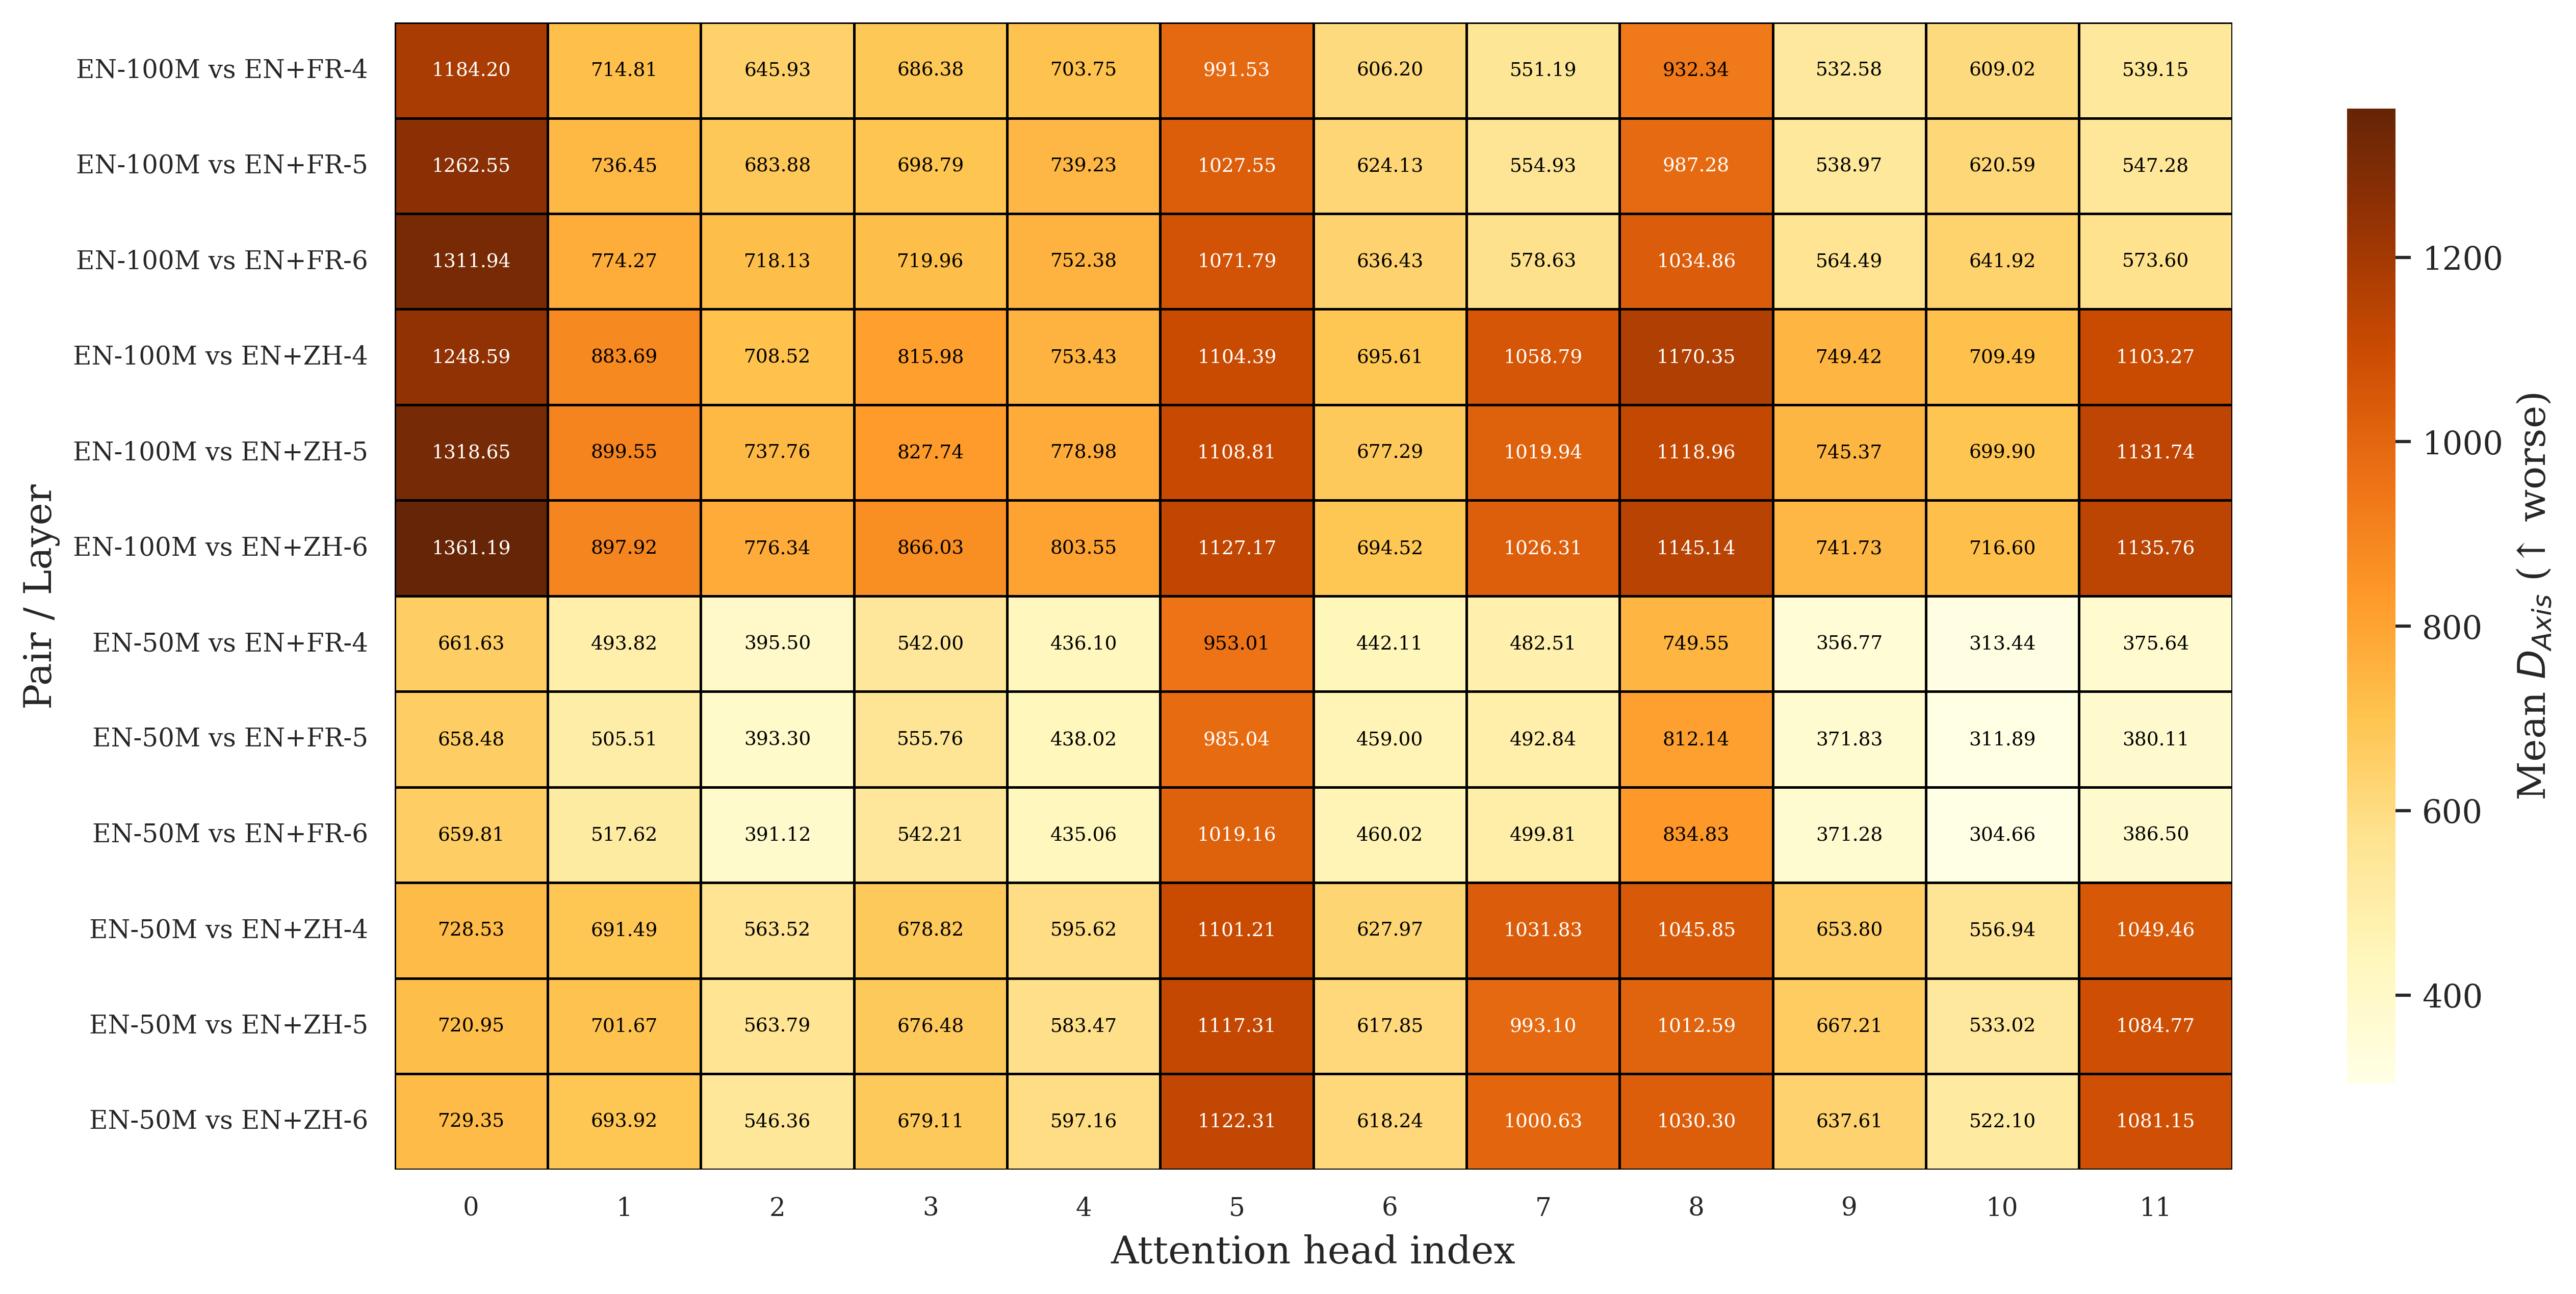
\includegraphics[width=0.95\textwidth]{figures/appendix_perhead_heatmap.png}
\caption{Per-head proxy analysis on middle layers (4--6). Each cell reports mean $D_{Axis}$ for a head-width channel slice; divergence is heterogeneously distributed across heads.}
\label{fig:appendix-perhead}
\end{figure*}

\begin{table}[t]
\centering
\scriptsize
\resizebox{\columnwidth}{!}{\begin{tabular}{@{}llrr@{}}
\toprule
Pair & Layer & Head & Mean $D_{Axis}$ \\
\midrule
EN-100M vs EN+ZH & 6 & 0 & 1361.193 \\
EN-100M vs EN+ZH & 5 & 0 & 1318.653 \\
EN-100M vs EN+FR & 6 & 0 & 1311.939 \\
EN-100M vs EN+FR & 5 & 0 & 1262.553 \\
EN-100M vs EN+ZH & 4 & 0 & 1248.585 \\
EN-100M vs EN+FR & 4 & 0 & 1184.204 \\
EN-100M vs EN+ZH & 4 & 8 & 1170.354 \\
EN-100M vs EN+ZH & 6 & 8 & 1145.142 \\
EN-100M vs EN+ZH & 6 & 11 & 1135.758 \\
EN-100M vs EN+ZH & 5 & 11 & 1131.744 \\
EN-100M vs EN+ZH & 6 & 5 & 1127.168 \\
EN-50M vs EN+ZH & 6 & 5 & 1122.307 \\
\bottomrule
\end{tabular}
}
\caption{Top per-head proxy cells by mean axis divergence.}
\label{tab:appendix-perhead-top}
\end{table}

\subsection{Additional Stratified and Word-Level Diagnostics}
\begin{figure*}[t]
\centering
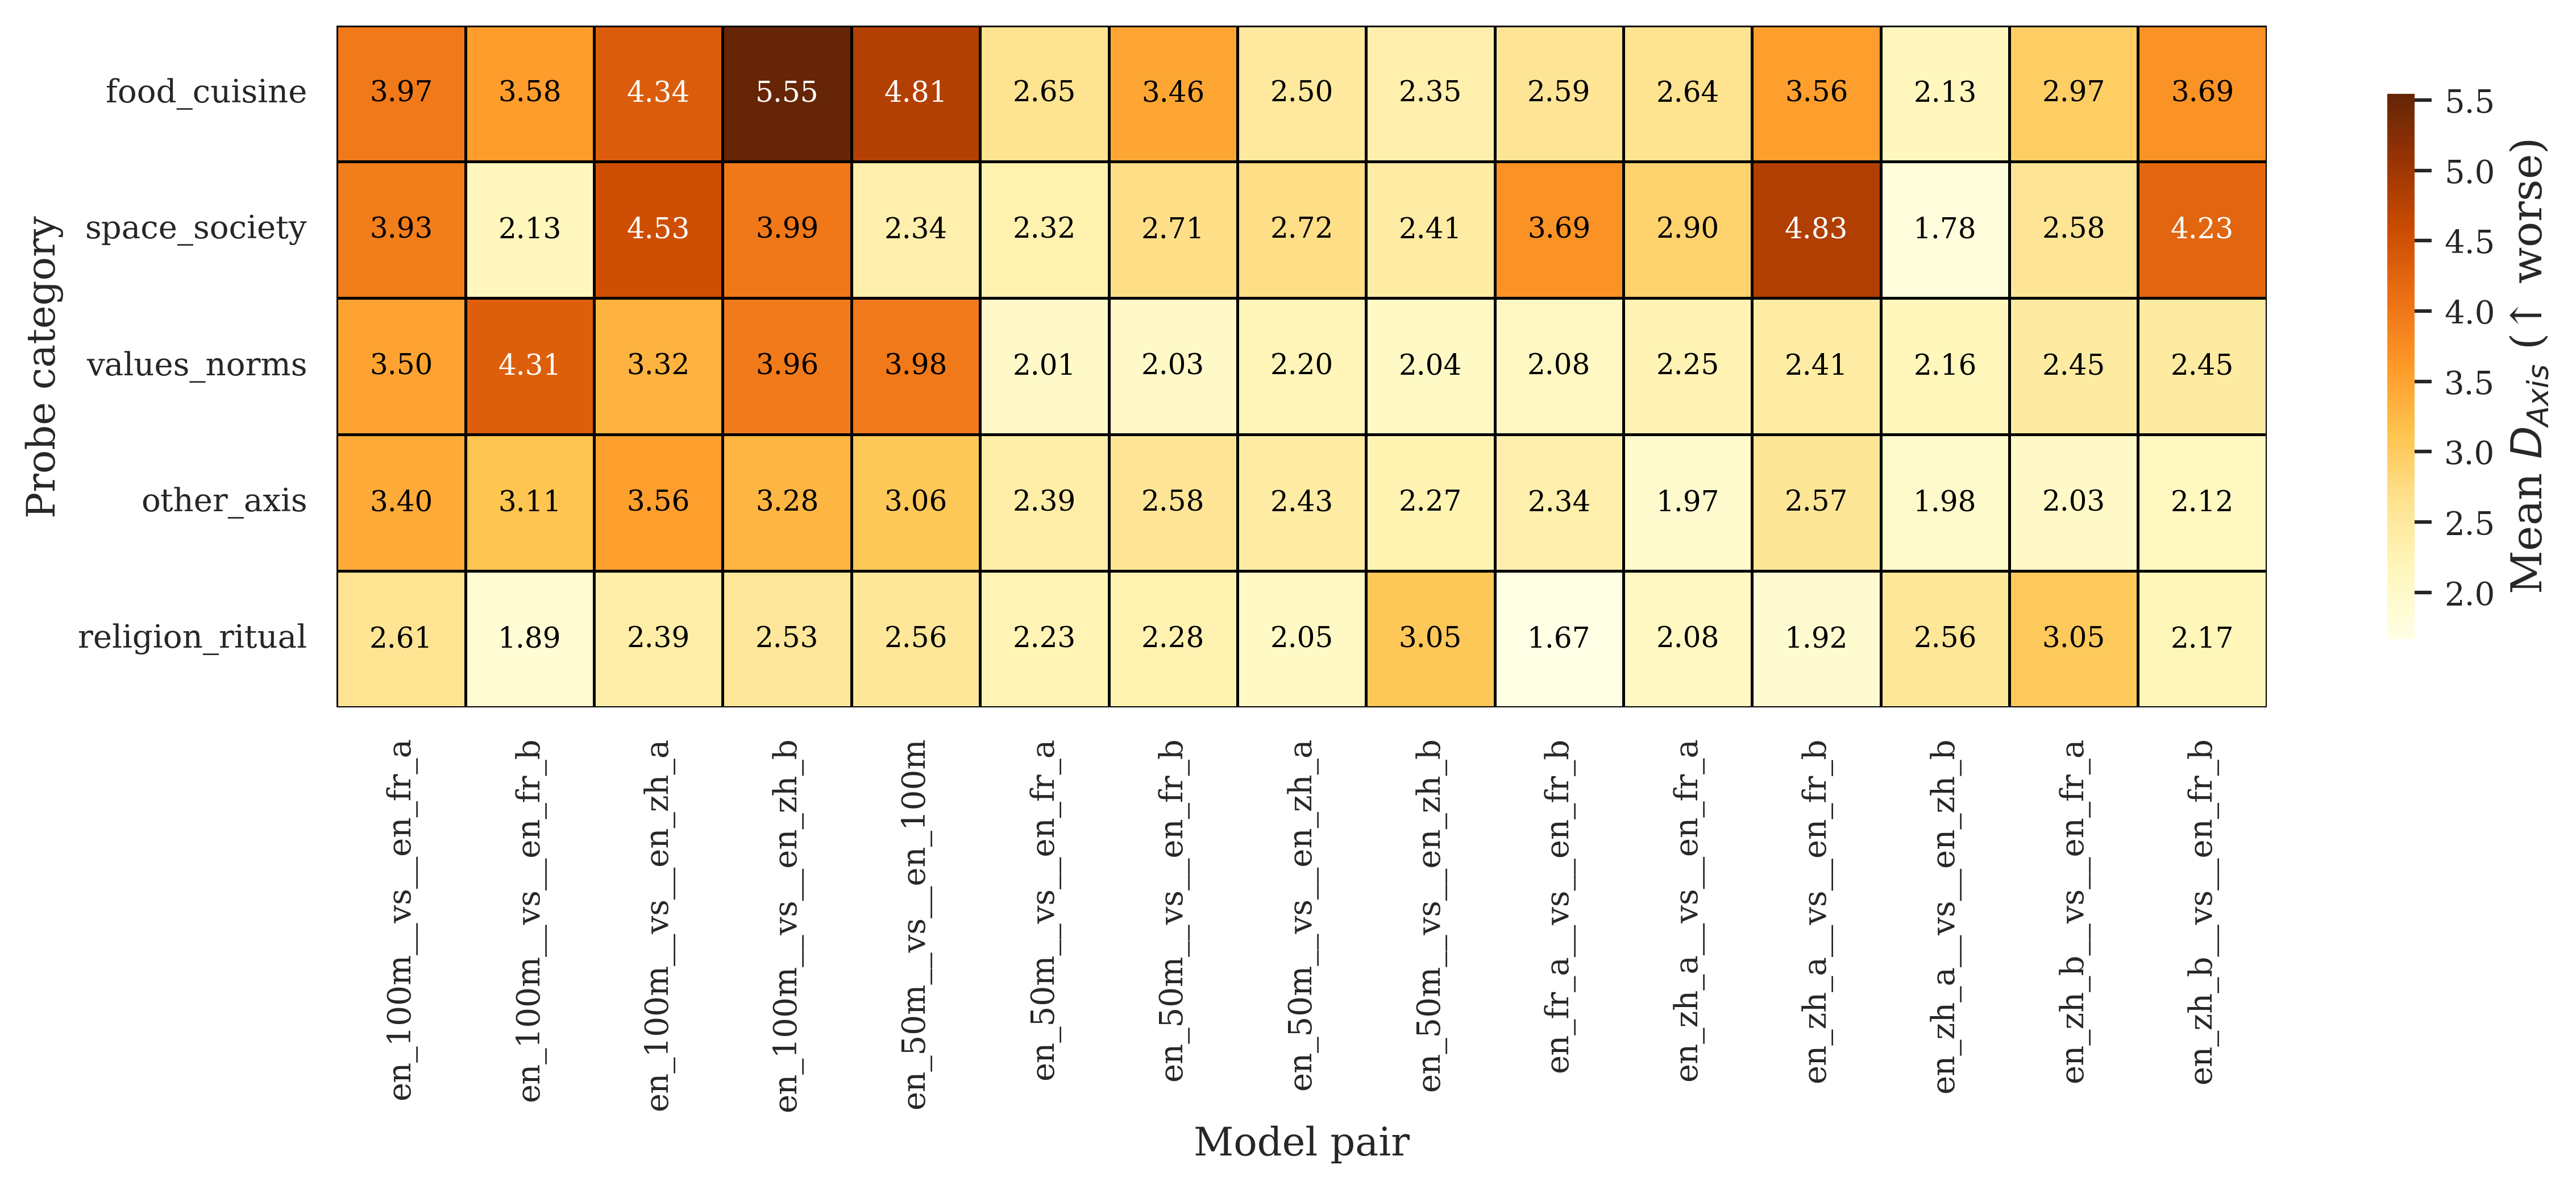
\includegraphics[width=0.95\textwidth]{figures/category_heatmap.png}
\caption{Category-stratified contextual axis divergence across model pairs.}
\label{fig:appendix-category-heatmap}
\end{figure*}

\begin{table}[t]
\centering
\scriptsize
\resizebox{\columnwidth}{!}{\begin{tabular}{@{}r l r r l r@{}}
\toprule
\multicolumn{3}{c}{Highest contextual divergence} & \multicolumn{3}{c}{Lowest contextual divergence} \\
\cmidrule(lr){1-3}\cmidrule(lr){4-6}
Rank & Word & Mean $D_{NN}$ & Rank & Word & Mean $D_{NN}$ \\
\midrule
1 & clan & 1.000 & 1 & extended mother & 0.286 \\
2 & clothing & 1.000 & 2 & sacred mosque & 0.315 \\
3 & kurta & 1.000 & 3 & extended daughter & 0.317 \\
4 & bamboo & 1.000 & 4 & extended father & 0.327 \\
5 & karma & 1.000 & 5 & sacred saint & 0.331 \\
6 & stereotype & 1.000 & 6 & sacred scripture & 0.341 \\
7 & nun & 1.000 & 7 & extended child & 0.347 \\
8 & folklore & 1.000 & 8 & extended grandfather & 0.356 \\
9 & mediation & 1.000 & 9 & sacred religion & 0.356 \\
10 & espresso & 1.000 & 10 & sacred monastery & 0.359 \\
\bottomrule
\end{tabular}
}
\caption{Per-word contextual neighbor-divergence hot spots.}
\label{tab:appendix-hotspots}
\end{table}

\subsection{Non-English Language Snapshot}
\begin{figure*}[t]
\centering
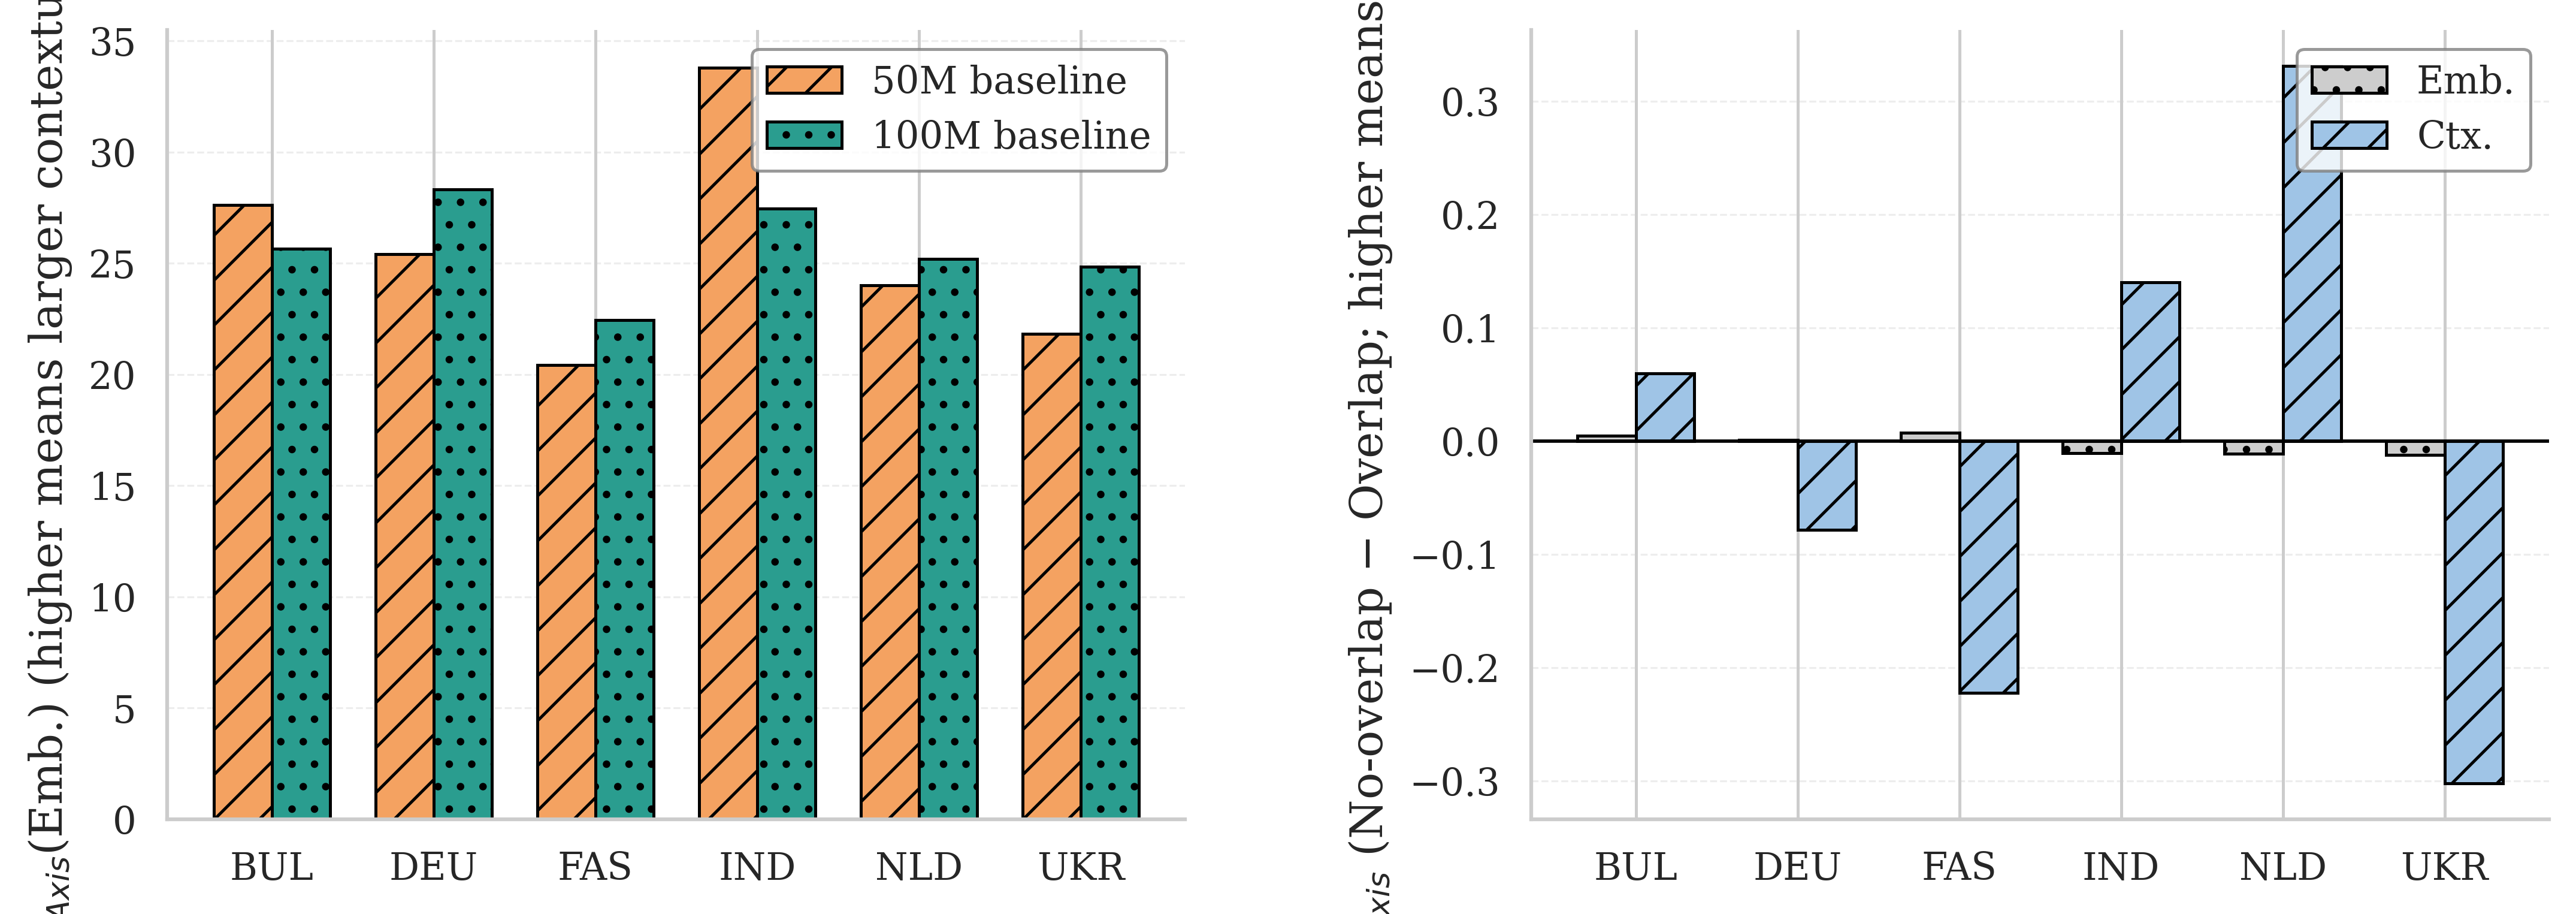
\includegraphics[width=0.95\textwidth]{figures/appendix_multilingual_overview.png}
\caption{Additional non-English language summary (FAS, NLD, UKR, BUL, IND, DEU). Left: contextual-to-embedding $D_{Axis}$ amplification ratios at $50$M and $100$M. Right: overlap-gain on axis divergence; contextual amplification dominates.}
\label{fig:appendix-multilingual-overview}
\end{figure*}

\begin{table*}[t]
\centering
\scriptsize
\resizebox{0.95\textwidth}{!}{\begin{tabular}{@{}lrrrrrr@{}}
\toprule
Lang & Ratio@50M & Ratio@100M & Gain $D_{NN}$ (Emb.) & Gain $D_{NN}$ (Ctx.) & Gain $D_{Axis}$ (Emb.) & Gain $D_{Axis}$ (Ctx.) \\
\midrule
BUL & 27.6$\times$ & 25.7$\times$ & 0.008 & 0.002 & 0.005 & 0.060 \\
DEU & 25.4$\times$ & 28.3$\times$ & -0.001 & 0.011 & 0.001 & -0.079 \\
FAS & 20.4$\times$ & 22.5$\times$ & -0.004 & 0.007 & 0.007 & -0.222 \\
IND & 33.8$\times$ & 27.5$\times$ & -0.002 & -0.009 & -0.011 & 0.140 \\
NLD & 24.0$\times$ & 25.2$\times$ & -0.011 & -0.017 & -0.011 & 0.331 \\
UKR & 21.8$\times$ & 24.8$\times$ & -0.006 & -0.005 & -0.012 & -0.302 \\
\bottomrule
\end{tabular}
}
\caption{Compact additional-language summary. Ratio@50M and Ratio@100M report contextual-to-embedding amplification for setup A. Gain columns report no-overlap minus overlap deltas averaged across baselines.}
\label{tab:appendix-multilingual-summary}
\end{table*}

\begin{table}[t]
\centering
\scriptsize
\resizebox{\columnwidth}{!}{\begin{tabular}{@{}llrrr@{}}
\toprule
Lang & Baseline & Mean ratio & CI low & CI high \\
\midrule
BUL & 100M & 25.7$\times$ & 22.4$\times$ & 29.1$\times$ \\
BUL & 50M & 27.7$\times$ & 23.4$\times$ & 32.2$\times$ \\
DEU & 100M & 28.3$\times$ & 24.4$\times$ & 32.4$\times$ \\
DEU & 50M & 25.5$\times$ & 21.9$\times$ & 29.2$\times$ \\
FAS & 100M & 22.4$\times$ & 18.9$\times$ & 26.2$\times$ \\
FAS & 50M & 20.5$\times$ & 17.2$\times$ & 24.0$\times$ \\
IND & 100M & 27.5$\times$ & 23.3$\times$ & 32.1$\times$ \\
IND & 50M & 34.0$\times$ & 28.4$\times$ & 39.7$\times$ \\
NLD & 100M & 25.2$\times$ & 22.0$\times$ & 28.6$\times$ \\
NLD & 50M & 24.1$\times$ & 20.6$\times$ & 27.7$\times$ \\
UKR & 100M & 24.9$\times$ & 20.7$\times$ & 29.4$\times$ \\
UKR & 50M & 21.9$\times$ & 18.5$\times$ & 25.6$\times$ \\
\bottomrule
\end{tabular}
}
\caption{Bootstrap 95\% CIs for contextual-to-embedding ratios in the additional-language slice, setup A at both baselines.}
\label{tab:appendix-multilingual-ratio-ci}
\end{table}

\begin{table}[t]
\centering
\scriptsize
\resizebox{\columnwidth}{!}{\begin{tabular}{@{}lr@{}}
\toprule
Quantity & Value \\
\midrule
OLS intercept & 28.621 \\
OLS coef: script-match (Latin=1) & 1.933 \\
OLS coef: family-match (Indo-European=1) & -4.895 \\
OLS coef: baseline(100M=1) & 0.150 \\
OLS $R^2$ (pooled 50M/100M; $n=12$) & 0.515 \\
Spearman $\rho$(distance proxy, mean ratio; $n=6$) & -0.207 \\
Spearman $p$-value & 0.694 \\
\bottomrule
\end{tabular}
}
\caption{Exploratory cross-language trend analysis. Pooled OLS uses ratio observations from both baselines; script-match and family-match are coarse binary proxies.}
\label{tab:appendix-multilingual-regression}
\end{table}

\begin{figure}[t]
\centering
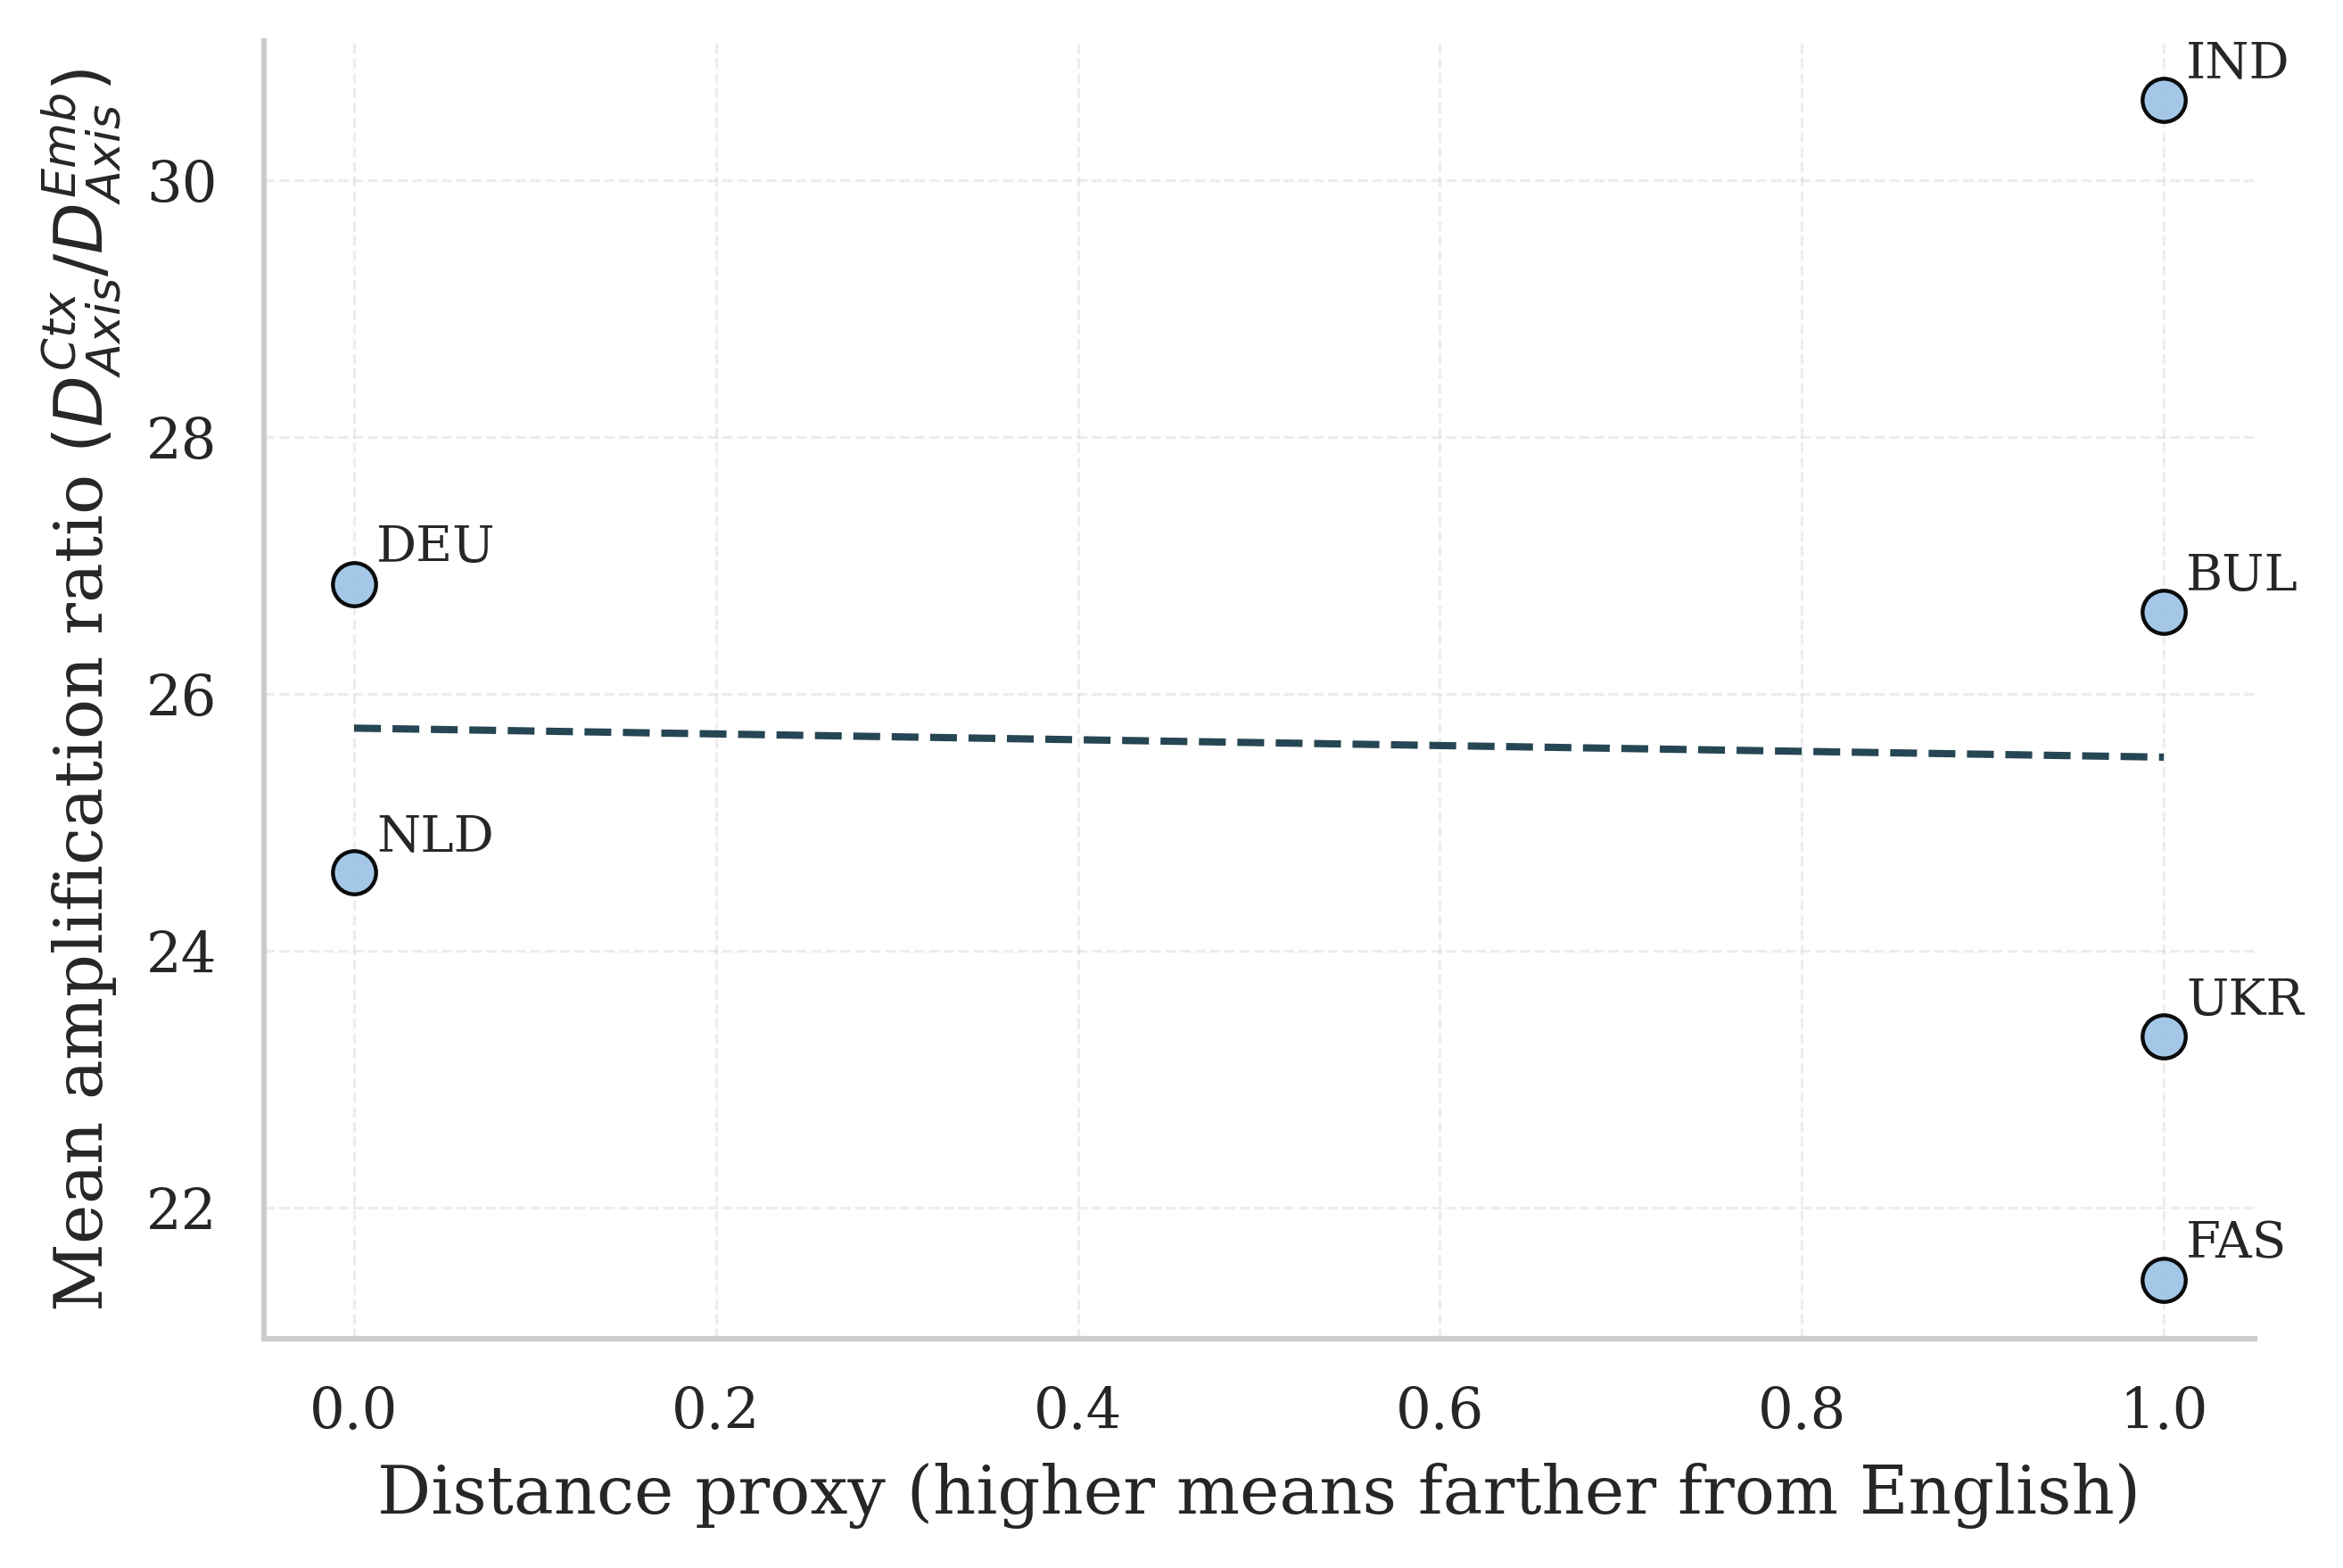
\includegraphics[width=\columnwidth]{figures/appendix_multilingual_regression_scatter.png}
\caption{Exploratory scatter: coarse distance proxy versus mean contextual-amplification ratio across additional non-English languages.}
\label{fig:appendix-multilingual-regression-scatter}
\end{figure}

\subsection{Planned Multi-Language Expansion Protocol}
Planned extensions will use a fixed language registry (language code, script family, typological metadata, cultural-distance metadata), fixed training geometry, fixed neutral-anchor alignment protocol, and fixed probe-construction/audit pipeline. This preserves comparability when extending beyond the current non-English target group.

\end{document}
